\documentclass[12pt]{article}
\renewcommand{\baselinestretch}{1.5}

\usepackage[top=1.5in, bottom=1.5in, left=1in, right=1in]{geometry}
\usepackage{algorithm}
\usepackage{algorithmic}
\usepackage[Sonny]{fncychap}
\usepackage{fancyhdr}
\usepackage{graphicx}
\usepackage{multirow}
\usepackage{verbatim}
\usepackage{pgfgantt}
\usepackage{pdfpages}
\usepackage[toc,page]{appendix}
\usepackage{url}
\usepackage{enumitem}
\usepackage[more]{tasks}
\usepackage{booktabs}
\usepackage{caption}
\usepackage{subcaption}
\usepackage{longtable}

\usepackage{titlesec}
\titleformat{\paragraph}{\normalfont\normalsize\bfseries}{\theparagraph}{1em}{}
\titlespacing*{\paragraph}{0pt}{3.25ex plus 1ex minus .2ex}{1.5ex plus .2ex}

\usepackage{hyperref}
\hypersetup{
    colorlinks,
    citecolor=black,
    filecolor=black,
    linkcolor=black,
    urlcolor=black
}

\usepackage{listings}
\lstset{
    breaklines=true,
    postbreak=\raisebox{0ex}[0ex][0ex]{\ensuremath{\color{red}\hookrightarrow\space}}
}

\NewTasks[style=enumerate]{enumeratecols}[\item](2)

\definecolor{PassGreen}{rgb}{0.0, 0.42, 0.24}

\begin{document}

% !TEX root = ../Report.tex

\begin{titlepage}
    \begin{center}
        \vspace*{0.6cm}
        
		\textbf{Using Location Data to Aid Recovery of Stolen Property}\\
		\vspace{5mm}
		\textbf{CS310 Computer Science Project}\\
		\vspace{5mm}
        \textbf{Naqash Tanzeel, 1314906}
        
        \vfill
        
\includegraphics[width=0.4\textwidth]{images/Warwick_Crest.png}
        \vfill
        
		Supervisor: Dr. Florin Ciuciu\\\vspace{6mm}
		Department of Computer Science\\ University of Warwick\\\vspace{6mm}
		2015-2016
    \end{center}
\end{titlepage}

\pagenumbering{roman}
% !TEX root =  ../Repport.tex

\begin{abstract}
	With technology advancing at an exponential rate and portable technology becoming more and more common, crime such as theft and burglary are at an alarmingly high level. Law enforcing agencies and insurance companies do their best to reunite owners with their valuables or compensate for them. However, if the power of the internet and community initiatives such as neighbourhood watch could be combined through an antitheft social network then crime could be combatted by citizens. A web application which allows users to store their possessions and tag them with a location could help people safeguard the things they value most. If these items are ever to be stolen then the owner can report this by tagging the item with the location it was stolen from and through the power of an online community the recovery of this item can be aided. Additionally, systems such as this protect users from becoming victims of fraud and if they become a victim of theft then the system can help simplify insurance claims. The system implements all this functionality, and more, as well as provide a basis for a live valuable tracking system which could transform the way that common people deal with crime.
\end{abstract}

\renewcommand{\abstractname}{Keywords}
\begin{abstract}
Social, Antitheft, Location, Recovery, Stolen, Valuables
\end{abstract}
\newpage

\renewcommand{\abstractname}{Acknowledgements}
\begin{abstract}
A lot of the work done in this project would not have been possible without the help of the stakeholder of the project. Firstly, a sincere thanks goes out to my project supervisor, Dr. Florin Ciuiciu, without whom this project would not exist and certainly would not be as successful as it has been. He provided the original idea and has continually provided much guidance throughout the initial planning, design and development process. Furthermore, his feedback on the project has helped to improve the final product and expand the project beyond its initial scope. Gratitude is also owed to all the users who assisted in the testing of the project and provided feedback, much of which was implemented, to improve the system since its first prototype.

Without the additional third-party frameworks and services, which reduced the development time, the project would not have been able to achieve all its goals. For this reason, credit is also owed to the companies and developers of these services. The largest of these companies include Google and Facebook. Finally, I would like to thank Taylor Otwell, the developer of the Laravel framework, which allowed the system to reach its full potential.
\end{abstract}

\newpage

\tableofcontents

\newpage
\listoffigures
\addcontentsline{toc}{section}{List of Figures}

\newpage
\listoftables
\addcontentsline{toc}{section}{List of Tables}

\newpage

\pagenumbering{arabic}
% !TEX root = ../Report.tex

\rhead{\small Using Location Data to Aid Recovery of Stolen Property}
\lfoot{\centering \thepage}

\chapter{Introduction}
\label{Chapter:Introduction}

Social media has been a rapidly growing industry in the 21st century, with the social network Facebook worth just under \$315 billion dollars as of May 2016 despite only being founded in 2004 \cite{Forbes:Facebook}. However, with the popularity of Facebook and other social networks such as Twitter and Instagram, numerous social issues have arisen which are yet to be fully addressed. Fidelis is an alternative to these networks, which attempts to address these issues. This specification discusses the requirements of the social network Fidelis, as well as the strategies which will be used to design, develop and then test the system.

\section{Problem Statement}
\label{sec:problemstatement}

\section{Project Aims}
Abuse detection, provision of user-specific content and reputation scoring are the three key features which can be implemented to ensure that a social network is trustworthy. Therefore, the aim of this project is to build a new social network called Fidelis, in order to demonstrate the methods which can be used to implement these features and to evaluate how effective the methods are in solving the issues which established social networks currently face when attempting to earn and retain the trust of their users.

\subsection{Abuse Detection}
As discussed in section \ref{sec:problemstatement}, abuse has played a large role in users losing trust in social networks. Therefore, Fidelis s be able to detect abusive content, which can then be hidden from the user. This will allow Fidelis to provide a platform for open discussion and debate without the threat of abuse and intimidation. However, what is perceived as abusive is dependent on the individual user, therefore how strict the detection algorithm is at identifying abuse must be flexible. In addition, traditional methods of handling abuse such as blocking users and reporting posts must still be implemented so that no abuse goes undetected. On the other hand, the user should also have the option to view content which has been flagged as abuse by the algorithm, so that the network does not enforce censorship on content which is posted. An exception is when the content posted is deemed illegal and therefore should be removed from the platform completely.

\subsection{Content Recommendation and Filtering}
Content which is provided to each user by a social network should be engaging for that user. Therefore, Fidelis should be able to recommend content which is known to interest the user. This does not necessarily mean that the posts/users provided agree with a user's point of view, because it is important the platform is able to stimulate debate so that it is representative of the real world. In order for the system to ascertain which topics a particular user is interested in, it should be able to detect the topics of the user's posts as well as the topics of posts which the user interacts with. In addition to recommending content, the user should be able to easily access new content. Therefore, Fidelis must provide feeds which are filtered based on their topics and provide post tagging, which allows users to explore posts addressing more specific topics.

\subsection{Reputation Scoring}
By determining the reputation of users, Fidelis should be able to determine the reliability of content and therefore tailor how visible it is on the platform. This requires for a score to be calculated for each user, which represents how reputable they are and therefore how worthwhile it would be to follow them. This score can then be used to determine which users should be recommended to others. The features which determine the user reputation are:

\begin{itemize}
\item Number of followers. If a user has a large number of followers, they would have a higher reputation score because it suggests that their content is worth following.
\item Number of votes. A user which receives a large number of votes posts more engaging content and is therefore more reputable.
\item Number of positive votes vs. number of negative votes. A user which posts more positively received content is more likely to be reputable.
\item Number of comments on their posts. As with the votes, the number of comments on a post can be used to determine how engaging the content is. Therefore users which receive more responses to their content have a higher reputation.
\end{itemize}

As well as scoring the reputation of each user, Fidelis should score the reputation of each post. This is because a reputable user may not always post content of the same quality. Therefore, the following features of a post are used to determine its reputation score:

\begin{itemize}
\item Number of votes.
\item Number of positive votes vs. number of negative votes.
\item Number of comments.
\end{itemize}

\section{Project Motivation}
As mentioned previously, the popular social networks of today have given rise to numerous social issues. One of these such issues is `trolling', with `The Guardian' reporting that ``one in four teenagers suffered hate incidents online last year'' \cite{Gani:Trolling}. 

The social networks' current failure to find an effective solution to these pitfalls of social media therefore offers the question of whether a network could be created, which tailors the content users see based on what that particular user would prefer to see. This does not only include filtering any abusive posts, but also not offering them content which is not of interest to them, either based on the theme of the content or who posted it.

\section{Project Stakeholders}
The internal stakeholders for this project are the development team - Isheanesu Gambe, Naqash Tanzeel, Thomas Mcaloone and Jordan Olney - and Dr Matthew Leeke, who is the project supervisor. To ensure the project is successful, the wider public will also be involved to offer feedback on the progress of Fidelis throughout the duration of the project. In order to test the system, data from other social networks will be required to populate the database with realistic posts. Therefore, the Twitter accounts of multiple stakeholders, both external and internal, will be used, so that large quantities of data can be collected in a short period of time, without exceeding the rate limits imposed by the Twitter API.

\section{Report Structure}
The purpose of this report is to provide a comprehensive account of the process undertaken whilst developing the system associated with the project. The report has been broke down into 3 main sections which identify the high level stages this project went through.

\paragraph{Research and Analysis}
An introduction to the problem being faced and combatted, motivations behind the undertaking of this project and an analysis of any stakeholders is presented in chapter \ref{Chapter:Introduction}. Chapter \ref{Chapter:Research} discusses and analyses any existing solutions, along with any technologies that may be used throughout the project, listing their advantages. Chapter \ref{Chapter:Issues} briefly discusses any issues that may arise and must be considered, whilst chapter \ref{Chapter:SystemRequirements} outlines the original and final requirements for the system.

\paragraph{Development and Testing}
Chapter \ref{Chapter:Design} discusses the thought process behind the designing of the system, whilst chapter \ref{Chapter:Implementation} details the implementation of the system. Chapter \ref{Chapter:Testing} outlines the testing procedures that were carried out, prior to, throughout, and post development. Collectively chapters \ref{Chapter:Design}-\ref{Chapter:Testing} cover the development process from start to finish.

\paragraph{Evaluation and Reflection}
The final 3 chapters reflect on the entire process of developing the system. Chapter \ref{Chapter:ProjectManagement} discusses the project management strategies employed to tackle the project whereas chapter \ref{Chapter:Evaluation} provides an analysis of the work carried out and how well it satisfies the initial requirements of the project. Finally, chapter \ref{Chapter:Conclusion} concludes with a summary and any suggestions for extending the system further.

\chapter{Research}
\label{Chapter:Research}
Social media sites have become integral to daily life in today's society. It is difficult for new ideas to gain popularity and draw users from their established social networks. Even for social media juggernauts like Facebook and Twitter, user retention is a challenge currently being faced. This has driven the need for the addition of innovative features to existing systems, such as the ability to use virtual reality headsets for viewing images and videos \cite{Facebook:VR}. To be able to achieve the goals set out for Fidelis, it was imperative to look at existing systems and build on what they have done successfully, but also identify their downfalls and improve upon these. Additionally, research into a number of techniques that can address these downfalls and provide Fidelis users with security and comfort was done.

\section{Related Work}
The following sections discuss the research done on the four core Fidelis functionalities: abuse detection, content filtering, recommendations and reputation scoring. Each section discusses the given topic and looks at a number of different approaches for each.

\subsection{Abuse Detection}
Basic abuse detection on social media platforms consists of rudimentary techniques such as flagging content deemed offensive or through the existence of content moderators. However, for more advanced methods most abuse detection systems employ natural language processing (NLP) and machine learning techniques to detect abusive user content. It is common to build a machine learning classifier that has the ability to classify content as abuse or not. For the purposes of this report, we will focus on user posts on a social media site. These classifiers learn from a given collection of abusive posts, and use the resulting model to classify future posts. Classifiers vary in the features extracted from posts to determine whether they are abusive. The success and accuracy of classifiers hinges very much on the selected features, making feature selection an important part of building the classifier.

As with any system that attempts NLP, the difficulty in detecting abusive posts lies within the intricacies of the English language. The task of identifying abusive content is unfortunately not as simple as a keyword search, and needs some understanding of underlying language structure and consideration for its linguistic features. As identified by Nobata et al in their research, \cite{nobata2016abusive}, when abusive language is used online it is purposefully obfuscated to the lessen the chance of it being detected. This, coupled with the seemingly popular use of ``text speech'' makes the simple task of detecting \emph{shit} much harder when a system faces (arguably) creative variations like \emph{shieeeeeet}. Abuse obfuscation also does not necessarily have to focus on the word itself, but can instead be hidden in the delivery of the message. Perfect grammar and spelling can be used just as effectively, if not more, to mask the true meaning behind a message. This again highlights the inefficacy in just using keywords. With just this approach,
\begin{equation}
\label{eq:rude}
\mbox{\textsl{The USA is exemplifies what happens when you let a filthy ape become president}}
\end{equation}
would go unpunished even though it is evidently abusive. Challenges faced when detecting abuse are not only from correctly identifying abusive posts, but are also from avoiding the misclassification of non-abusive posts. Profanity can be used for abuse, emphasis, playfulness or frustration. We are only interested in profanity being used for abuse, and as such the remaining use cases need not be detected. 

Features commonly extracted from natural language to perform abuse detection are syntactic and lexical features. Syntactic features look at words alone, and explore the relationships between words in a sentence \cite{liao2010large}. This can be seen in part-of-speech tagging, which tags a word in a sentence based on its syntactic class . Words in different contexts would be tagged differently, which leads to dis-ambiguity when processing words. Using semantic features, we can identify the relationship between \textbf{he} and \textbf{dog} in the following sentence:
\begin{equation}
\label{eq:semantic}
\mbox{\textsl{The dog ran after the ball; he really enjoyed playing games with his owner.}}
\end{equation}
Comparatively, lexical features treat each word or phrase as an individual entity, meaning word patterns can be found in sentences by the appearance of words and their frequencies \cite{chen2012detecting}. An example lexical feature is the stemmed version of a word. Stemming reduces all occurrences of words to a ``root'' word \cite{Elastic:Stem}. So in the above example, the root for \emph{enjoyed} would be \emph{enjoy}. 

In their work on an abuse detection classifier, Nobata et al \cite{nobata2016abusive} use syntactic and lexical features, in addition to n-gram, linguistic and distributional semantic features. 3-5 character n-grams are used to identify abusive language that has been obfuscated by elongating the original word (\textsl{lol} becomes \textsl{looooool}). Whereas n-gram features are used to detect directly abusive words, syntactic features are used to capture long-range dependencies between words using dependency parsing. So in \ref{eq:semantic}, the dependency president and ape is identified. Through the combination of these features, the resulting classifier is able to detect hate speech, derogatory and profane language.

Ravazi et al to build an automatic flame detection system \cite{razavi2010offensive}, where content is deemed as flame if its main intention is attack (hate speech, racism, extremism, homophobia) or it contains abusive or hostile words, phrases or language. The system is built upon a three-level classifier. Each level extracts a set of features which are then used as the input for the next level. The first level uses the Complement Naive Bayes classifier to select the most discriminative features. The second level uses the Multinomial Update Naive Bayes Classifier. The third and final level uses DTNB, which is a rule-based classifier. The third level also makes use of an Insulting and Abusing Language Dictionary, which is a collection of words, phrases, and expressions, with different degrees of manifestation of flame varieties.

More recently, Chatzakou et al looked at identifying bullies and aggressive users on Twitter by characterising users based on user, text and network based features \cite{chatzakou2017mean}. Focusing on just the text-based features, word embeddings are used to capture the syntactic and semantic relation of words. In this embedding, the word2vec model \cite{mikolov2013efficient}, developed by Mikolov et al, is used to generate a vector representation for a given post, which it gets by averaging the vectors for each word in the post. This is coupled with the use of the SentiStrength tool \cite{SentiStrength:Home}, which estimates the positive and negative sentiment in short texts. These features alone would not suffice for abuse detection, but combined with user and network-based features provide a new and innovative way of approaching the problem of abusive language detection.

\subsection{Content Filtering} \label{sec:research-content-filtering}
As with the abuse detection, content filtering is a classification problem. Classification in this instance, however, is concerned with the automated categorisation of users pots. Each post is assigned to a topic based on post content. These categorised posts enable output to be presented as a set of filtered feeds, allowing users to easily locate content they find engaging. As with abuse detection, content filtering requires NLP, which presents challenges when selecting an appropriate machine learning model to be used as the classifier, along with determining features to use for model training.

Before considering the type of model to use, feature extraction must be used to represent posts in a way which allows a model to detect patterns. The most common method for textual content is Bag-of-Words (BoW), where ``a document is considered to be simply a collection of the words which occur in it at least once. The order of the words, the combinations in which they occur, paragraph structuring, punctuation and of course the meanings of the words are all ignored''~\cite{Bramer:BoW}. The loss of ordering in the content can result in some of the meaning of the post being lost. Despite this, ``BoW features are effective at capturing the general topic of the discourse in which the topic had occurred''~\cite{Jurafsky:BoW}.

With regards to the model itself, there are numerous models which perform classification, including support Na\"ive Bayes, vector machines (SVMs) and k-nearest neighbours, with each model having their own advantages and disadvantages.

Na\"ive Bayes assumes that each feature in the data is independent in order to calculate the maximum posterior given the training data~\cite{Kuncheva:Bayes}. This is done maximising the Bayes formula, where $c$ is the number classes and $i$ is each possible model:

\begin{equation}
\label{eq:bayes}
P(\omega_{i}|\mathbf{x}) = \frac{P(\omega_{i})p(\mathbf{x}|\omega_{i})}{\sum_{j=1}^{c}P(\omega_{j})p(\mathbf{x}|\omega_{j})}\quad i=1,...,c
\end{equation}

\noindent As we know features are independent, this substitution can be made to simplify the above equation:  
\begin{equation}
\label{eq:bayes-simple}
p(\mathbf{x}|\omega_{i})=\prod_{j=1}^{n}p(x_{j}|\omega_{i})\quad i=1,...,c
\end{equation}

\noindent ,where $n$ is the number of inputs. This simplification makes computation inexpensive, but the assumption may not necessarily hold with the posts on Fidelis. For example, the presence of one word in the BoW could increase the likelihood of another word being present, thus assuming independence may make the model less effective.

Conversely, SVMs uses a decision boundary to categorise data. The boundary ``is chosen to be the one for which the margin is maximized''~\cite{Bishop:SVM}, where the margin is the distance between the boundary and the nearest data points from each class. One possible difficulty with using SVMs is the choice of kernel, which is used to measure the similarity of two data points. This is because ``once the kernel is fixed, SVM classifiers have only one user-chosen parameter (the error penalty), but the kernel is a very big rug under which to sweep parameters''~\cite{Burges:SVM}.

K-nearest neighbours ``directly uses the data sample to estimate the density''~\cite{Zaki:KNN}. The performance of this model decreases as the dimensionality of the data increases, so due to the likely sparsity of the data which the model will be using in Fidelis, this could have a major implication on the effectiveness of the topic categorisation. Another drawback is that the use of k-nearest neighbours is ``computationally expensive''~\cite{Kuncheva:KNN}.

Since Fidelis will be required to categorise posts from the launch of the site, even when no posts currently exist, data must be collected from existing social media platforms, which can model realistic Fidelis posts. These posts must also be assigned a category each, so that the classifier can be trained on the data collected. As part of their paper `Harnessing Web Page Directories for Large-Scale Classification of Tweets', Zubiaga and Ji curated a set of Tweets, which were assigned one of the following categories: arts, business, education, games, health, home, news, recreation, science, shopping, society, sport and technology ~\cite{Zubiaga:Tweets}. The dataset has been made publicly available so can be used to train the classifier.

\subsection{Content Recommendation}
As previously mentioned, the public is demanding more from social media platforms in terms of how they interact with and are engaged by them. In recent years there has been a welcomed increase in the application of recommender systems. Recommender systems provide item recommendations that might be of interest to a user \cite{ricci2011introduction}. Originally used on music and video streaming services like Spotify and Netflix, recommender systems have permeated to social media platforms. The challenge faced when recommending new items to a user is that there is no guarantee that the user will like the content. Research has therefore focused on tailoring and personalising recommendations to a given user. To this end, most recommender systems implement either content or collaborative-based filtering algorithms.

\subsubsection{Collaborative-based Filtering} 
Under collaborative-based filtering algorithms, users are recommended new content based on the opinion of other like-minded users, or using information from content rated by a user \cite{sarwar2001item}. Recommendations take the form of either predictions, which are numerical values that represent how likely it is for a user to like an item they have not previously liked, or as a list of $N$ items a user will like the most \cite{sarwar2001item}. Such algorithms can be memory-based, building a network of neighbours around a user who have a history of agreeing with the user \cite{sarwar2001item}, or model-based, whereby a machine learning approach is taken and item recommendations are viewed probabilistically.  common approach to collaborative-based filtering is to build an $N \times N$ user similarity matrix. Each entry in the matrix corresponds to the similarity score between user $u_i$ and $u_j$. This is illustrated in \ref{example:similarity-matrix} for a system with three users. User similarities are calculated using a number of different methods, but the most similarity measure used is cosine similarity \cite{linden2003amazon} \cite{sarwar2001item} \cite{liu2014new}. Other similarity measures used include mean square difference (Eq. \ref{eq:msd}) and Jaccard similarity (Eq. \ref{eq:jacard}) \cite{liu2014new}. Similarity between users is determined by each users item-vector.

\begin{align}
msd(\mathbf{A}, \mathbf{B}) = \frac{1}{N}\sum\limits_{i=1}^{n}(A_i - B_i)^2 \label{eq:msd} \\
jacard(\mathbf{A}, \mathbf{B}) = \frac{\mathbf{A} \cdot \mathbf{B}}{\|\mathbf{A}\|^2 + \|\mathbf{B}\|^2 -  \mathbf{A} \cdot \mathbf{B}} \label{eq:jacard}
\end{align}
Vectors are created from items rated by a user, allowing the similarity between two vectors to be measured. Item-based collaborative filtering can be used as a replacement for user-based filtering. This variant on collaborative filtering provides recommendations based on item similarities. Items that a user has previously rated are scored against ``unseen'' items, and a user is presented with a list of the top $N$ recommendations \cite{sarwar2001item}. Similarity can  again be determined using either cosine or conditional probability-based calculations. Alternatively, with conditional probability-based similarity two items are similar if the probability that a new item will be consumed given another item already consumed by the user is high \cite{sarwar2001item}. The conditional probability is calculated based on the frequency of an item, where frequency for an item $X$ is the number of users that have consumed or rated $X$. 

\begin{equation}
\bordermatrix{~ & u_1 & u_2 & u_3 \cr
            u_1 & - & 0.76 & 0.83 \cr
            u_2 & 0.76 & - & 0.6\cr
            u_3 & 0.83 & 0.6 & - \cr}
\label{example:similarity-matrix}
\end{equation}

\subsubsection{Content-based Filtering} 
Content-based filtering algorithms measure correlation between the content of ``candidate'' recommendation items and items previously rated by a user \cite{van2000using}. This is the only major difference between the two filtering approaches. Similarly to collaborative-based filtering, similarity between a ``candidate'' item and a user is calculated using the same similarity measures, and again using a vector of features for a given item. Features composing each item vector vary, but common techniques to extract textual features include:
\begin{itemize}
\item Bag of Words (BoW) \cite{vanetti2010content}, a text classification technique where a piece of text is represented as a multiset, with grammar and word ordering disregarded \cite{scikit:bow}
\item Term Frequency-Inverse Document Frequency (TF-IDF) \cite{van2000using}, where terms (or words) are assigned a weight based on how often they appear in a particular document and how frequently they occur across the entire collection of documents \cite{scikit:tfidf}
\end{itemize} 

\subsection{Reputation Scoring}
Trust is an imperative across all social networks. Different networks choose to model user trust in different ways, with some networks choosing to follow an explicit trust model (if user A trusts user B, B also trusts A), and others preferring an implicit model (user A can trust User B, but trust is not necessarily reflexive). In regards to Fidelis, trust will be based upon reputation scores for both users and the posts they make. Having these scores attached to each user on the network will allow users to make informed decisions on who they choose to engage with. By building a circle of trust around themselves, users will be able to create a network of others with whom they can reliably engage with positively.

One interesting way to explore the idea of reputation scoring is through the use of collaboration-based reputation. In their paper, McNally et al explore the idea of modelling user reputations through collaboration events \cite{mcnally2013}. Collaboration events are events that occur when users provide feedback on the content posted by other users. This feedback, for example in the form of voting on a post, is used in a calculation to determine how much the user giving feedback trusts the original poster. From these collaboration events, a collaboration graph can be created where nodes in the graph correspond to the original poster and users who provided feedback on the post. Trust scores are represented as edges in the graph, and are aggregated to calculate the reputation of individual users using ``Weighted-Sum'' and ``Page Rank'' scoring metrics \cite{mcnally2013}.

Zacharia et al explore the application of collaborative reputation mechanisms used in electronic markets for wider use. Two mechanisms for scoring user reputations are discussed which can handle both loosely and highly connected online communities. The first, Sporas \cite{zacharia2000}, handles scoring reputations in a loosely connected community. Under Sporas, users have a single reputation which is updated according to feedback provided by other users. New users start with the minimum reputation value, and as a user’s reputation grows they experience smaller changes in their reputation after each update. The second mechanism, Histos \cite{zacharia2000}, is a pairwise rating system. These pairwise ratings between users are modelled through a directed graph, with nodes in the graph representing users and ``weighted edges between nodes representing the most recent reputation given by one user to another, with the arrow pointing towards the rated user.'' \cite{zacharia2000}.

\section{Existing Systems}
There are a range of existing system which provide a similar service or a subset of the services described in the project aims. However these solutions have all been designed to tackle different problems and all have their respective drawbacks. In order to avoid facing problems that have been solved by these services, an analysis is carried out to discuss the advantages and shortcomings of each service. Using this, a superior social network which implements the advantages of these services whilst tackling the disadvantages can be be designed.

\subsection{Facebook}
``Founded in 2004, Facebook's mission is to give people the power to share and make the world more open and connected''~\cite{Facebook:About}. Since its launch, it is the most popular social network to date and boasts an active user base of approximately 1.7 billion people~\cite{Statista:Facebook}. According to Facebook, people use the social network ``to stay connected with friends and family, to discover what's going on in the world, and to share and express what matters to them''. Facebook users must register before using the social network and are free to create a personal profile in order to interact with other users which they can add as friends. Furthermore, Facebook users may join user groups based on workplace, college or school and can also categorise their Facebook contacts into lists. Users can post status updates or other content and message each other~\cite{Statista:Facebook}. 

The Facebook friend system operates on a mutual trust basis. This means if person A and person B are friends on Facebook because person A wishes to see content from Person B then person B implicitly trusts person B and also sees content from person B. However, Facebook later realised that mutual trust is not always implicit of a friendship and added a following and unfollowing feature. As of this update, if two users are friends then they are automatically following each other but they can optionally unfollow one another, meaning that they will still have a friendship but will not see content from one another. This adds the concept of a one way trust relationship which Fidelis aims to implement on an explicit level which the user has control over and an implicit level which filters content automatically through the use of reputation.

\subsection{Twitter}
Twitter is an online social networking and microblogging service, which allows registered users to read and post `tweets'~\cite{Statista:Twitter}. Twitter posts are limited to a short 140 characters and can either be posted on the users timeline or sent directly to users as messages. If a user chooses to make their account public then anyone can view their timeline and browse their tweets. Twitter is one of the most popular social networks worldwide with 313 million monthly active users~\cite{Statista:Twitter, Twitter:About}. Part of the appeal is the ability of users to follow any other user, with a private or verified public profile, enabling users to interact with celebrities or friends who regularly post on the social media site.

Unlike the Facebook friend system, Twitter operates purely on a following system. This means if user A wishes to follow user B, given user B has a public profile, user A will see all of the content shared by user B but the same will not apply vice versa until user B also chooses to follow user A. The success of the system lies in this core functionality which allowed popular figures to create accounts that could be followed by the mass public, enabling a one way stream of communication. Twitter also introduced another popular feature, the concept of adding `hashtags` to tweets, which allows tweets to be categorised into popular topics. This can then be used to increase activity by recommending trending topics to users. However, one thing Twitter does not handle effectively is abuse detection and spam filtering which results in increased `trolling` activity on public profiles, and even bullying. Fidelis will inherit the core functionality of Twitter but extend it to include abuse detection and content filtering so that users are not inundated content but instead receive very personalised and engaging content.

\subsection{Reddit}
Reddit is a forum-based social network that `bridges communities and individuals with ideas, the latest digital trends, and breaking news'~\cite{Reddit:About}. It works by allowing users to create boards and sub-boards known as sub-reddits. Once a sub-reddit has been created, users can start threads which anyone may read but only registered users can post replies to. The system was designed to allow users to ask questions where a large community can leave answers. A user may reply to a reply or a reply of a reply. The social network was launched in 2005 and, according to statistics from August 2016, has approximately 243 millions unique monthly visitors~\cite{Statista:Reddit}.

Like most social networks, Reddit also has a way of rating and categorising posts. However, unlike the others, Reddit uses a voting system that allows users to explicitly dislike content and change the quality score. Categorising in Reddit is done through sub-reddits, meaning users must explicitly go and post content in the appropriate category rather than content being automatically categorised. The advantage of this approach is that categories are maintained by users and should always be up to date. Content inside these categories is then ordered by the overall score (number of up votes - number of down votes). A similar approach to this will be employed when scoring content on Fidelis along with some other scores contributing to the order of posts on a feed.

\section{Technologies}
\label{Section:Technologies}
When developing a web application, it is important to explore the range of technologies already available in order to speed up the development process. For this reason, several third party technologies were used to provide some of the core functionality of the system. These technologies include but are not limited to jQuery, Laravel and Google Maps. In addition to the third party technologies, the latest web development technologies were also employed to provide the essential and basic functionality of a web application.

\subsection{Web Technologies} \label{Section:Web_Technologies}

\begin{figure}[H]
  \centering
  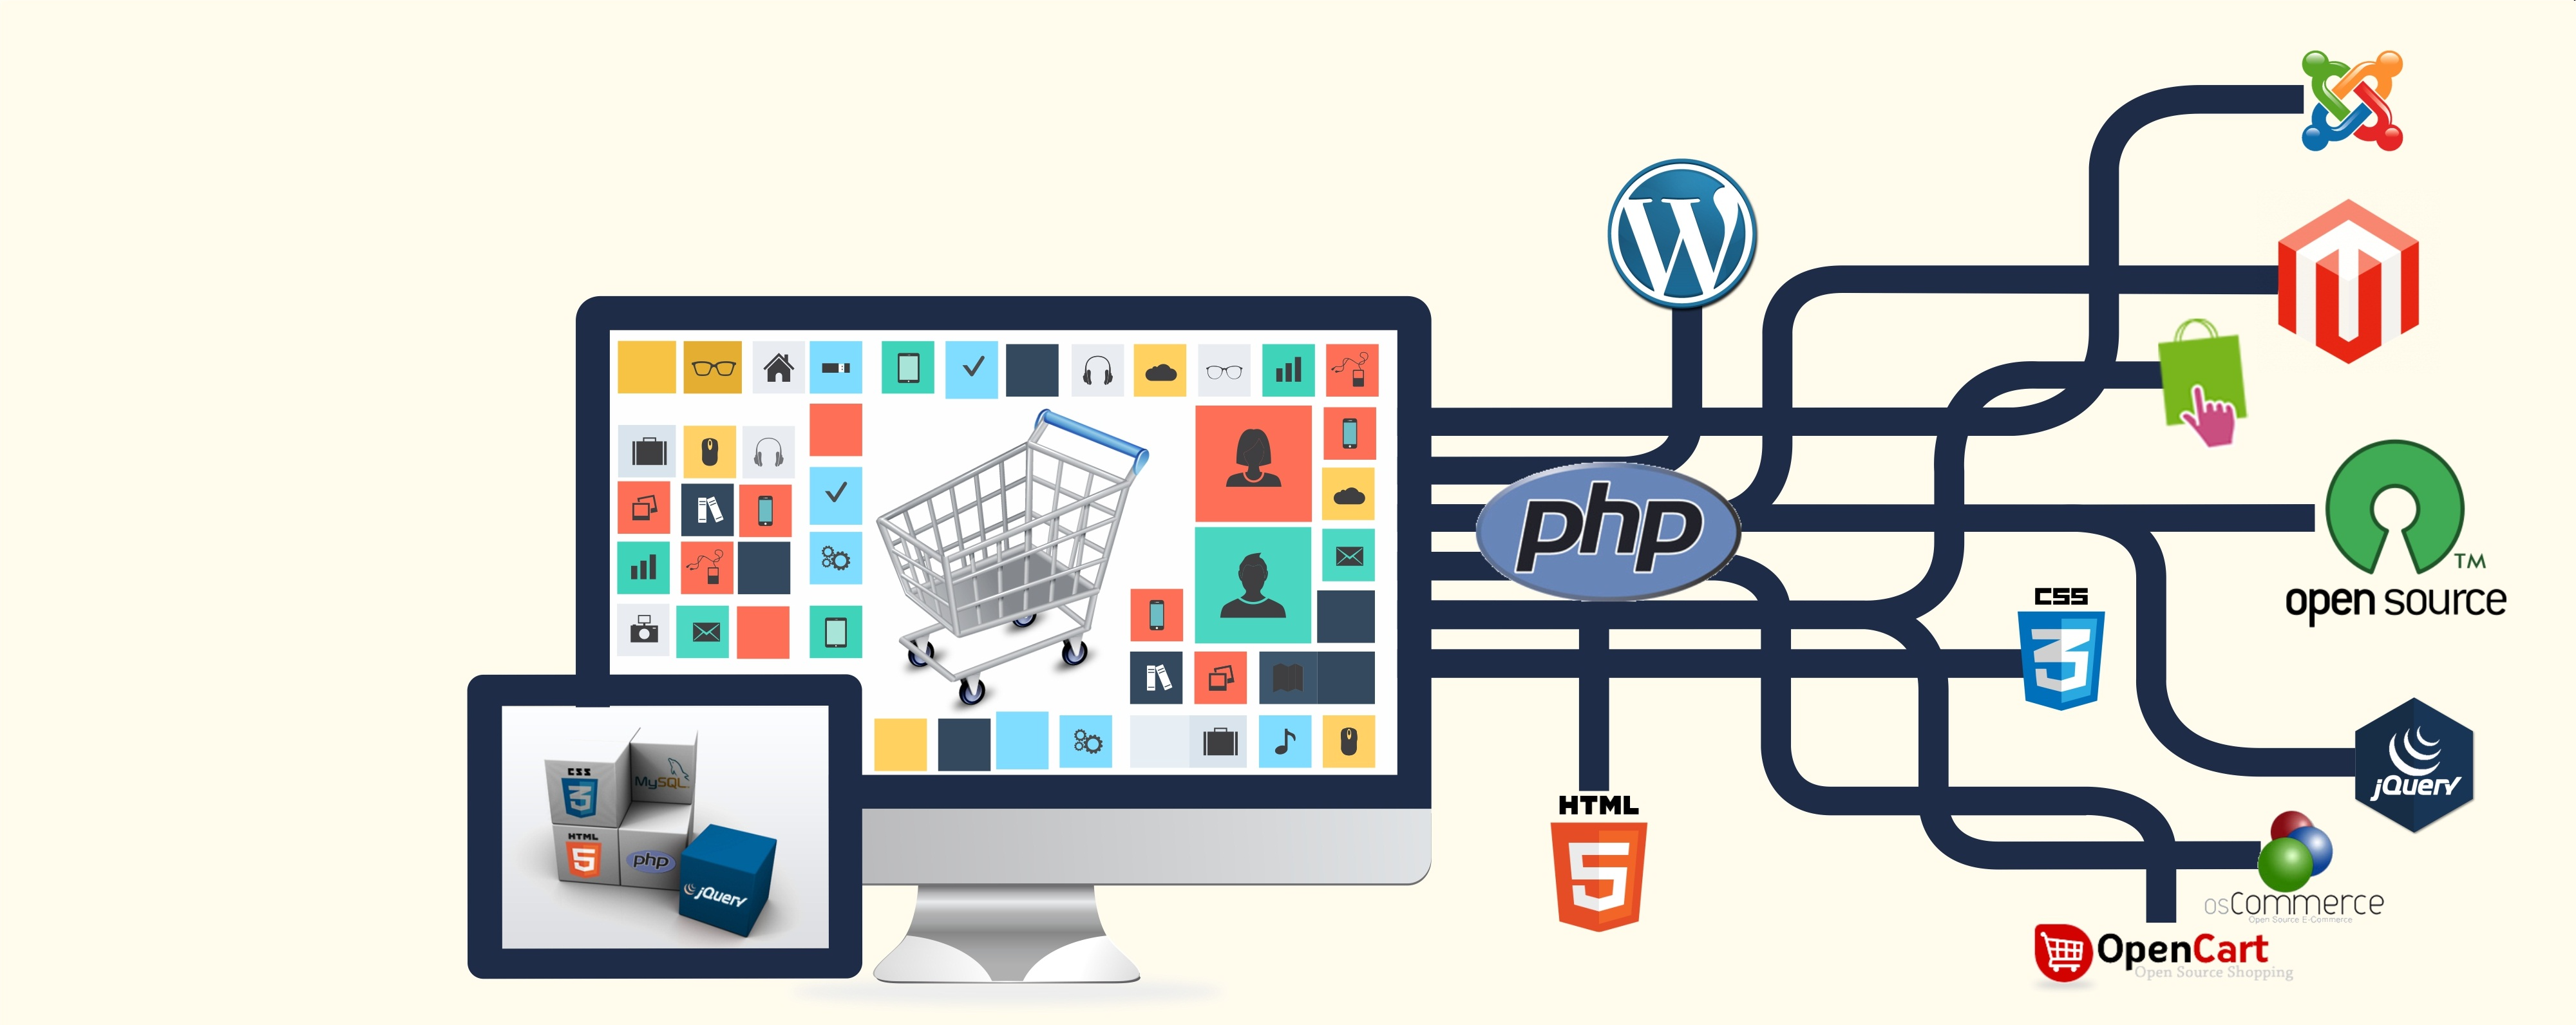
\includegraphics[width=1.0\textwidth]{Images/Research/Technologies/WebTechnologies}
  \caption{Information Exchange in an MVC Application.} \label{fig:WebTechnologies} 
\end{figure}

There are many web technologies for getting a website up and running, as illustrated in figure \ref{fig:WebTechnologies}. These range from the traditional HTML, CSS, JavaScript and PHP to newer and other languages such as Python, Java, and Ruby \cite{Differential:WebTechnologies}. Some of these technologies were researched and have been analysed below as they will most likely be employed for the development process.

\subsubsection{HTML} 
Hyper Text Markup Language (HTML) is a markup language used for structuring and presenting content on the world wide web \cite{W3:HTML5}. HTML 5 is the recommended standard by W3 as of October 28, 2014 and as such will be used to structure the web application being developed. HTML in itself cannot be used to change the style of page as it was only designed for defining the structure of a page but fortunately HTML tags can be styled. 

\subsubsection{CSS} 
Cascading Style Sheets (CSS) is a simple mechanism for adding style (e.g. fonts, colours, spacing) to Web documents \cite{W3:CSS}. CSS3 is the latest evolution of the Cascading Style Sheets language and aims at extending CSS2.1. It brings a lot of long-awaited novelties, like rounded corners, shadows, gradients, transitions or animations, as well as new layouts like multi-columns, flexible box or grid layouts \cite{Mozilla:CSS3}. CSS3 is being used in this project as it provides a much larger range of styles which are required by Bootstrap.

\subsubsection{JavaScript}
JavaScript (JS) is a high-level, lightweight, interpreted, programming language with first-class functions \cite{Mozilla:JavaScript}. Although JavaScript is not a necessary requirement, it offers many advantages such as allowing manipulation of the document structure after the page has been loaded. As a result of this, one can add, remove or animate content on the page. Inarguably, the main advantage of JavaScript is that it is interpreted on the client side which means less processing is done on the server. This allows for faster loading times as parts of the document can be loaded later, on demand, when required. Collectively, all these and more features improve the user experience and provide a good reason to incorporate JavaScript into a web app.

\subsubsection{PHP} 
``PHP is a popular general-purpose scripting language that is especially suited to web development'' \cite{PHP:Home}. It is fast, flexible and pragmatic, and powers everything from a blog to the largest and most popular websites in the world \cite{PHP:Home}. One of the main advantages of using PHP is that it allows for untyped variables which is particularly useful for fetching records from the database as the attributes of a tuple will be of different types. Other advantages of PHP being the ability to write Object-Oriented code, particularly useful when implementing the frameworks discussed below.

\subsection{Frameworks}
\begin{figure}[H]
  \centering
  
\includegraphics[width=1.0\textwidth]{Images/Research/Technologies/WebFrameworks}
  \caption{Open Source Web Frameworks Built Around Popular Web Technologies for Developers.} \label{fig:WebFrameworks} 
\end{figure}

Frameworks significantly reduce the amount of code that needs to be written to get a project up and running and hence allow the developer to prototype with speed. A range of frameworks are available, as illustrated in figure \ref{fig:WebFrameworks}. Some of these will be employed to develop the projects and have been discussed in depth in this section.

\subsubsection{Model-View-Controller (MVC)}
Initially, as stated in the project specification, the system was to be designed as a web based application implemented using the four basic web technologies mentioned previously in section \ref{Section:Web_Technologies}. After completing the initial setup and some implementation, this approach was challenged and a decision was made to find an alternative approach. One of the main reasons for this change in approaches was the overwhelming amount of code that was duplicated across pages making it difficult to make changes whilst maintaining consistency across the pages. As a result, it was decided that a Model-View-Controller approach should be used and implemented using an existing framework.

\begin{figure}[H]
  \centering
  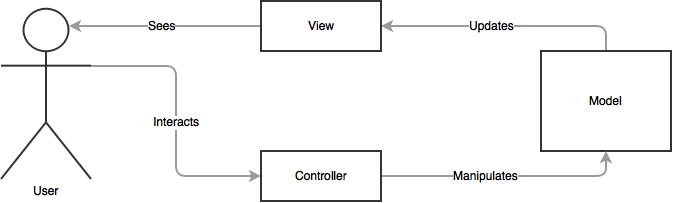
\includegraphics[width=1.0\textwidth]{Images/Research/Technologies/MVC}
  \caption{Information Exchange in an MVC Application.} \label{fig:MVC} 
\end{figure}

The Model-View-Controller (MVC) pattern separates the modelling of the domain, the presentation, and the actions based on user input into three separate classes \cite{MSDN:MVC}. A description of each section as well a graphical representation of communication, figure \ref{fig:MVC}, is given above.

\begin{itemize}
	\item \textbf{Model.} The model manages the behaviour and data of the application domain, responds to requests for information about its state (usually from the view), and responds to instructions to change state (usually from the controller) \cite{MSDN:MVC}. In essence the model is responsible for all interaction with the database and contains any code that either queries or updates records in the database along with some output formatting.
	\item \textbf{View.} The view manages the display of information \cite{MSDN:MVC}. The advantage of this approach is that repeated content can be split into separate views with placeholders and then included by passing in parameters to fill the placeholders. This means that the developer only needs to change the code in one place, particularly useful for things such as navigation and foorter which are consistent across pages.
	\item \textbf{Controller.} The controller interprets the mouse and keyboard inputs from the user, informing the model and/or the view to change as appropriate \cite{MSDN:MVC}. This is where majority of the logic and PHP code for the application is written. Any algorithms and data pre-processing or post-processing methods are written inside the controller.
\end{itemize}

\subsubsection{Laravel}
Laravel, an open-source PHP web application framework intended for the development of web applications following the MVC architectural pattern, developed by Taylor Otwell, was chosen after researching various frameworks \cite{Laravel:Home}. Laravel was chosen over other frameworks for a number of reasons. Not only does it provide an implementation of the MVC pattern, but it also allows allows the user to define custom routes and decide where each route leads rather than having the URL be determined by the file path. Additionally, Laravel comes with solutions to a lot of common tasks and problems straight out of the box making it easier to develop the system straight away without having to ``reinvent the wheel''.

\subsubsection{jQuery} 
jQuery is a fast, small, and feature-rich JavaScript library \cite{jQuery:Home}. It will be used over standard JavaScript as it makes things like HTML document traversal and manipulation, event handling, animation, and Ajax much simpler with an easy-to-use API that works across a multitude of browsers \cite{jQuery:Home}. Although jQuery doesn't necessarily provide any additional functionality over JavaScript as it is powered by JavaScript, it provides shorter notations for common JavaScript functions and provides implementation of features that are lacking in JavaScript, or take long to implement. It can be setup and used by simply including a single script in the document.

\subsubsection{Bootstrap} 
Bootstrap is the most popular HTML, CSS, and JS framework for developing responsive, mobile first projects on the web \cite{Bootstrap:Home}. The main advantage of using Bootstrap is that it easily and efficiently scales your websites and applications with a single code base, from phones to tablets to desktops with CSS media queries. Additionally Bootstrap comes with a whole range of HTML, CSS and jQuery components, that have been pre-styled, further speeding up the development process.

\subsection{Storage}
One of the most fundamental parts of the system is retaining the data that the users enter into the system. There are two different storage solutions for storing and querying the data provided by users. These are both discussed below.

\subsubsection{MySQL} 
MySQL is an open source database management system used for managing data held in a relational database management system (RDBMS) \cite{MySQL:Home}. An SQL database will be used to store all textual information entered by the users. This includes user information, location data, item details and any other necessary information. SQL databases are not encrypted and hence any user credentials such as password will be stored in an encrypted format to prevent access to user accounts in case of a breach.

\subsubsection{Resources}
Along with textual input, it is also necessary to store the images associated as photos with posts, uploaded by the users. One approach to this could be to convert the file to binary and store the binary data in the SQL database. However this approach would lead to the database rapidly growing in size and in turn affecting the performance. Not only would queries take longer to execute but also increase page load times due to the large record sizes. Another approach would be to store any uploaded files either on a storage server or on the web server so they are available on demand. This would result in faster loading time for pages containing these resources as they do not have to be transferred over the network. Due to this, the latter approach will be used during development.
\chapter{Legal, Social, Ethical and Professional Issues}
\label{Chapter:Issues}
With any system that involves human interaction, there are always a number of legal, ethical, social and professional issues that can arise. Due to the scope of this project and the amount of interaction by humans that may be involved, it is critical to be aware of the possible issues that could occur and find a way to address them.

\section{Legal Issues}
It is of vital importance that actions are taken to conform as closely as possible to both local and international laws. It is important to be completely clear with all stakeholders what is expected of them and what the terms of service, policies and procedures for the platform entail.

\subsection{Sensitive Data}
Since the proposed system focuses on users creating and sharing content, it is difficult to control what users may be posting. The platform is intended to promote an environment for free speech and sharing ideas/opinions, however there may be cases where a user publicly shares some information which was intended to be private or confidential. This could be personal information, or information pertaining to a third party such as an employer. Once information has been shared in this way there is little recourse; as soon as it is public, anyone can view it. In such a case one may argue that since the information was posted and shared through the Fidelis platform, the liability is with the platform and not with the user. It is therefore important to make it clear through policies and procedures that users are responsible for any content that they post or share through this platform. In a similar way, the use of unauthorised third party trademarks or copyright-protected works may be used by an individual in a way that infringes on the trademark/copyright. Users should therefore also be made aware that they are liable for any such infringement and that their posts may be removed due to this.

\subsection{Licensing}
Just as third-party materials posted to a social media site may infringe copyright or trademarks, posting photographs and video without proper releases may violate the privacy or publicity rights of individuals. Additionally, within certain industries, employees must ensure that they do not violate specific privacy regulations of their employer in their activities on social media sites. This phenomena should, however, be combatted by the combination of trust/reputation-based content filtering and the ability for users to report content.

\subsection{Resources}
In addition to ensuring users respect and uphold copyright and trademarks, it is important that the platform itself does not make use of and unlicensed materials. This includes, but is not limited to, using copyright-free images and ensuring that the required permissions are fulfilled for any software used in the creation and running of the platform. These guidelines were clearly relayed to all project team members to ensure no legal violations occurred.

\subsection{User Protection}
For all users of the Fidelis platform there is a responsibility to ensure that they are being treated fairly and legally. A common trend across many social media platforms is targeted `abuse' towards a specific individual. This can be in the form of `cyber bullying', `trolling’ or in some extreme cases, defamation. Defamation is defined as ``A false statement or fact, not made under privilege, that is communicated to a third person and that causes damage to a person’s reputation. For public figures, the plaintiff must also prove actual malice.'' \cite{BusinessLawToday}. Fidelis is focused on filtering the content that is presented to a user, which is intended to reduce the amount of negative content the user will see. While very negative content will be hidden from many users, the posts will still persist on the platform and so any content considered defamatory is still subject to defamation law. It should therefore be possible to delete these posts if needed as well as possibly using the posts to find the IP address or some other information about the original poster (i.e. to aid authorities whilst following both the law and any policies regarding privacy or anonymity of the user).

\subsection{International Law}
One particular legal pitfall to consider is local vs. international law. Social networks often have users posting from many different countries all over the world. A social media platform may adhere to all pertinent local laws in the country it was created in, however complications may arise due to unforeseen and possibly conflicting laws if the platform is operating in another country. With a vast number of legal jurisdictions, it can be difficult to keep up with international law, however there are some practical things that can be done to maintain a stronger legal position. For example, serving only select countries by limiting the selection of language options, or even by restricting the IP addresses of visitors to only allow users from specific countries \cite{Olswang}.

\section{Social Issues}
Despite one of the main features of Fidelis being abuse detection, it is important to consider the implications should certain abusive posts go undetected. Due to the nature of social media and the difficulty to systematically detect the semantics of a post, it is likely that there will be posts which are not detected by the abuse algorithms. As a result, functions such as being able to block a user and delete posts must be included, in the event a user does receive abusive content.

As well as abusive content, further offensive content may be posted on the site which does not fall under the category of abuse. This includes nudity and links to inappropriate or illegal content. As with abusive content, the user will be able to remove content from their feed which they find offensive, but in extreme cases users may have to be reported to the authorities or removed from the Fidelis site altogether.

In addition to abusive content, Fidelis would also be subject to other social issues which have been recognised with preexisting social networks. This includes possible mental health implications of socialising online instead of face-to-face. Research has suggested that ``digital communications less able to lower depression risk'' in comparison with ``people who regularly met in person with family and friends''~\cite{OHSU:Depression}. Therefore, it is important that Fidelis attempts to mitigate this risk by encouraging users not to spend too much time on the social network in its `Terms of Use' and also offers support by providing contact details of relevant helplines for those who seek help.

\section{Ethical Issues}
As a social media platform, there is a level of ethical responsibility to protect users by ensuring an agreed upon level of privacy. For example it is fairly common for company HR departments to review the social media pages of both job candidates and current employees. While this practice may be of use to the company, the design of the Fidelis platform is such that users should feel comfortable posting and discussing content without feeling the need to censor themselves. The user may not wish for everybody to see their posts and so as a compromise the user will be able to make their account private, preventing non-approved users from seeing the content they share.

This system aims to provide a platform for users to post and share content relating to a wide range of topics. In some cases, for example with politics, there are often issues that see people taking very different viewpoints. To provide a balanced platform for conversation and debate on these topics, it is crucial to take an unbiased approach to how the system decides which content to show to a user and which users to recommend to each other. It would be very easy for a person designing such a system to implement bias based on their own opinions, presenting all users with the same content that only shows one side of an argument. This would defeat the point of the Fidelis platform and be taking advantage of the user’s trust, so clearly these tactics will not be employed. All content suggestion will be based upon user preference above anything else.

\section{Professional Issues}
For the Fidelis to be able to function, it will be required to store large amounts of user data. It is therefore necessary to ensure that the privacy of the users is protected, by abiding by the `Data Protection Act' of 1998. This legislates that data is ``fairly and lawfully processed; processed for limited purposes and not in any manner incompatible with those purposes;
adequate, relevant and not excessive; accurate and where necessary, up to date; not kept for longer than is necessary; processed in line with the data subject's rights; secure and that personal information shall not be transferred to countries outside the EEA without adequate
Protection''~\cite{DPA}. So that the Fidelis system meets these requirements it is paramount that measures are taken to secure the database and to minimise corruption to the data, as well as regularly maintaining the data to remove anything which is surplus to the requirements of the system.
\chapter{System Requirements}
\label{Chapter:SystemRequirements}
No system can be developed without a direction. The requirements for a project guide the developer through the development process and ensure that core functionality is provided. These requirements are split into functional and non-functional requirements. Additionally, the requirements allow for a thorough testing plan to be implemented which can then later be used to evaluate the final product. 

\section{Requirement Refinement}
``Any project’s requirements need to be well thought out, balanced and clearly understood by all involved, but perhaps of most importance is that they are not dropped or compromised halfway through the project'' \cite{ReQTest:Requirements}. As the design and development of the project progressed, it became clear that some of the existing requirements, as defined in the project specification, would have to be refined as they were not sufficient to provide clear guidelines for development. Additionally, some of the requirements laid out in the specification were either optimistic or redundant and hence also required modification. As a result of this, several requirements were altered throughout development, some of which were changed numerous times. Throughout the refinement process the stakeholders of the project were consulted before any of the requirements were altered, added or removed. Fortunately, due to previous research, the requirements were reasonably accurate and did not require any major changes. The changing requirements could easily be integrated due to the agile development methodology, which provides opportunities to assess the direction of a project throughout the development lifecycle and make any changes through prototyping \cite{Agile:Home}.


\section{Functional Requirements}
The functional requirements will guide the development of all aspects of the system. These requirements will ensure that the system provides the necessary functionality, the implementation details of which are entirely up to the developer and may change during the development process.
\begin{enumerate}[label=\textbf{F\arabic*}]
	\item The system must be able to communicate with a number of third party APIs in order to retrieve data.
		\begin{enumerate}
			\item The system must be able to convert all data received from third parties into a consistent format.
		\end{enumerate}
	\item Users must be able to register and log into the system.
	\begin{enumerate}
		\item Registration may be done through manually entering all the required details or by using a third party which provide oAuth 2.0 services, such as but not limited to Facebook and Twitter.
		\item These credentials should be stored, in an encrypted format, so that they can later be used for authentication.
		\item Users should be able to recover their account in the case that they have forgotten their password or their account has been compromised.
		\item A user maintains the right to be able to delete their account publicly, however this data may still be retained privately.
	\end{enumerate}
	\item A user may make their account private, preventing other users from being able to see the content they share.
		\begin{enumerate}
			\item If a user attempts to follow a private account, a request to follow is sent to the private user and must be approved before the relationship is created.
		\end{enumerate}
	\item A user may block another user.
		\begin{enumerate}
			\item If the blocked user is already following the blocking user, then they automatically unfollow the user.
			\item Once a user has been blocked, the blocked user should not be able to find the blocking users profile through search or otherwise.
			\item If a user has blocked a user then they may also unblock the user. This will not restore any previous following relationships.
		\end{enumerate}
	\item In order to see content, users should be able to add other users to their ��trust circle��.
		\begin{enumerate}
			\item This is identified as a one way relationship in which ��user A follows user B�� implies that ��user A trust user B��.
			\item Similarly, if users no longer wish to see content from specific users then they may unfollow a user they are already following.
		\end{enumerate}
	\item The system will overcome the cold-start problem, under which a user will not see anything on their timeline upon registration, by providing a set of predefined categories which can be used to explore.
		\begin{enumerate}
			\item Users are able to access a customised `Discover' feed by subscribing to categories, sub categories or topics.
			\item The `Discover' feed will then be generated by pulling content from the various subscriptions allowing the user to explore topics based on their interest, discover new content as well as new users who they may follow.
		\end{enumerate}
	\item The system will provide a personal feed where the user is able to view content from the people they trust, prioritised by the reputation of the people they follow as well as the reputation of the content itself.
		\begin{enumerate}
			\item The user may hide content from their personal feed which they find offensive, or just uninteresting. This should be used to learn and adapt the recommendation system by modifying the posters reputation.
		\end{enumerate}
	\item A user must be able to post new content onto the system.
		\begin{enumerate}
			\item A post may include text, images or videos. Additionally an image or video post may also contain text.
			\item When posting content, users may optionally tag the post or leave it untagged.
			\item When the user tags a post with a popular topic, e.g. \#Brexit, the post should automatically be assigned to the correct category, e.g. Politics in the aforementioned case, using a bucket of keywords per category.
			\item If a tag is mentioned and the post cannot be categorised automatically then the user may be prompted to assign one of the predefined categories so that the system can learn and adapt for the future. Additional processes may be used to verify that tags are correctly classified.
		\end{enumerate}
	\item Users can view any text, photo or video posts made by public accounts or by private accounts which they follow.
		\begin{enumerate}
			\item Viewing media content should open up in a popup or similar so users can view the post and comment on it.
		\end{enumerate}
	\item Users must be able to reply to a post made by another user.
		\begin{enumerate}
			\item If the user has made their account private then only users following the author of the post may comment on or see the post.
		\end{enumerate}
	\item Users may interact with content they come across by liking, disliking or sharing it. Each of these actions will impact the reputation of the content.
		\begin{enumerate}
			\item The user should also be able to reverse their interaction, e.g. un-liking a liked post.
		\end{enumerate}
	\item The system will automatically calculate a reputation score for users which symbolises the trustworthiness of the user and the content they post.
		\begin{enumerate}
			\item This score will be impacted by a range of factors. For example, a user'��s trustworthiness increases as their number of followers (people who trust the user) goes up. Similarly, this reputation can also decrease if the users content is disliked.
			\item This will be used, along with other factors such as mutual connections, to recommend other users the user may be interested in following.
		\end{enumerate}
	\item The system will also calculate a reputation for each user posted content to represent the quality of content.
		\begin{enumerate}
			\item As other users react to the content by liking, disliking or sharing it, the reputation of the post will change which in turn impacts the author's reputation.
			\item Highly scored posts will be more likely to be recommended to other users on the `Discover' or `Categories' pages.
		\end{enumerate}
	\item Each user will be able to choose how the reputation is calculated and how the notion of trust is implemented.
		\begin{enumerate}
			\item This feature will be available through the settings menu. Each algorithm will use different properties of a user and posts to compute the score.
			\item Additionally, the user will be able to change the sensitivity of the scoring system from mild to strong.
		\end{enumerate}
	\item The system will incorporate abuse detection to prevent things such as profanity, swearing and nudity amongst other things.
		\begin{enumerate}
			\item Each user can adjust the sensitivity of their abuse detection system depending on which content they would like to hide.
			\item Due to the processing requirements, this may be implemented as a job which executes at regular interval to remove content.
		\end{enumerate}
	\item Users can report content which they find is inappropriate or offensive, such as profanity or nudity.
		\begin{enumerate}
			\item The report along with the reported content is sent to a moderation system. This report must be picked up by a moderator who either dismisses the reported if the content adheres to the guidelines or the content is removed and the user's reputation is changed to reflect this.
		\end{enumerate}
\end{enumerate}

\section{Non-Functional Requirements}
In order for the system to be successful and used, it is essential that it is available on demand, regardless of time and place. This means that the system must support a range of devices varying from desktop to small hand-held smartphones. The non-functional requirements for this project will not only help to ensure that the systems operates smoothly and provides a responsive user experience, but also ensure that the development of the system is up to a high standard.
\begin{enumerate}[label=\textbf{NF\arabic*}]
	\item \textit{Compatibility}: The system must be cross browser compatible and support all devices with a modern browser.
		\begin{enumerate}
			\item A responsive design and structure must be used to ensure the system is compatible with all devices.
			\item The following categories of devices must be well supported.
			\begin{enumerate}
				\item Mobile
				\item Tablet
				\item Desktop
			\end{enumerate}
			\item Functionality should not be limited or restricted on any of the given devices but may be implemented differently
		\end{enumerate}
	\item \textit{Usability}: The system must be intuitive and user friendly.
		\begin{enumerate}
			\item The system must be intuitive and easy to navigate. Users must be able to access pages without any guidance.
			\item The user experience across all pages must be consistent in terms of design and functionality.
			\item The user must never encounter errors, but if the system encounters an error then an appropriate output should be produced.
			\item Appropriate user feedback must be given when interacting with the system.
			\item The system must have an appropriate load time across all pages.
			\begin{enumerate}
				\item Studies have shown that nearly half of the users consider abandoning a site if it takes longer than 3 seconds to load ~\cite{Kissmetrics:Speed}.
			\end{enumerate}
		\end{enumerate}
	\item \textit{Security}: The system and the data held must be secure.
		\begin{enumerate}
			\item The users details and credentials, such as email and password must be appropriately secured.
			\item Any data added by the user or associated to the user must only be available to the user unless explicitly made available to the public.
			\item Users may not have access to personal information about other users, such as email address and location data.
			\item Any resources uploaded by the user must not be browsable by other users, unless made public by the user.
		\end{enumerate}
	\item \textit{Scalability}: The system must be scalable and respond well to growth.
		\begin{enumerate}
			\item Data storage and processing decisions must be made whilst taking growth and expansion into consideration.
			\item Growth should not limit functionality and availability - the system must be able to cope with this.
			\item As storage and processing can be costly, these must be considered when developing the system so efficient use is made of both of these resources.
		\end{enumerate}
	\item \textit{Extensibility}: The system must be extensible and support further development.
		\begin{enumerate}
			\item The system must be designed modularly, regardless of whether it may need changing or not.
			\item Design decisions must be made with extensibility and growth in mind and as a result, any component or part of the system must be easily replaceable with an upgrade.
			\item Each of these components must be independent and operate independently.
		\end{enumerate}
	\item \textit{Maintainability}: The system must be maintainable.
		\begin{enumerate}
			\item Standard and good code practices should be adhered to whilst developing the system.
			\item A version control system should be used to make regular checkpoints.
			\item The system and any external resources or technologies should always be kept up-to-date to avoid any issues.
			\item Any hardware decision made must take maintainability into consideration.
		\end{enumerate}
	\item \textit{Readability}: The system must be well documented
		\begin{enumerate}
			\item The codebase must be thoroughly documented using any standard commenting conventions and guidelines for the specific language.
			\item Any progress logs must provide a clear outline of the progress and changes made.
			\item Version control commits must detail the changes made - any addition or removal of features must be clearly stated.
			\item A clear outline of the system and its functionality must be provided.
		\end{enumerate}
\end{enumerate}

\section{Limitations and Constraints}
As with all systems, there exist constraints which will limit the capability and the performance of the system. The development server, which the system is currently being developed and tested on, is hosted on a local machine as resources and performance are not a significant issue for development purposes. The production version of the system is being deployed on a Virtual Private Server (VPS) provided by DigitalOcean \cite{DigitalOcean:Home}. The VPS has limited resources and in turn, very minimal performance. The details of the local and deployed production server are listed in table \ref{table:ServerSpec} below.

\begin{table}[H]
	\centering
	\begin{tabular}{@{}ll@{}}
		\toprule
		\multicolumn{2}{c}{Local Server}       	\\ \midrule
		Resource         & Availability 			\\ \midrule
		CPU              & 2            			\\
		RAM              & 8 GB       			\\
		Disk Space (SSD) & 256 GB        		\\
		Bandwidth        & Unlimited      		\\
		Operating System & OSX     				\\ \bottomrule
	\end{tabular}
	\quad
	\begin{tabular}{@{}ll@{}}
		\toprule
		\multicolumn{2}{c}{Production Server}	\\ \midrule
		Resource         & Availability 			\\ \midrule
		CPU              & 1            			\\
		RAM              & 512 MB       			\\
		Disk Space (SSD) & 20 GB        			\\
		Bandwidth        & 1000 GB      			\\
		Operating System & Cent OS      			\\ \bottomrule
	\end{tabular}
	\caption{Local and Production Server Specifications}
	\label{table:ServerSpec}
\end{table}

As depicted by the table, the deployed VPS has very limited processing power, RAM and disk space. When a web server is installed, the processing power will limit the load time of web pages as the web server will only be allowed a portion of the resources. Additionally, the system relies on disk space for both hosting the database and storing resources uploaded by the users. The disk space will limit the amount of resources that can be stored and the amount of data that may be stored in the database. Fortunately, the data stored in the database is all textual and hence requires very minimal storage space. The one thing that the server is not limited by is the bandwidth, which is a huge 1TB per month.

The VPS currently runs CentOS, a Linux distribution that is stable, predictable, manageable and reproducible, derived from the sources of Red Hat Enterprise Linux (RHEL) \cite{CentOS:Home}. Although CentOS is a relatively light distribution, it will still consume a significant portion of the available resources and hence leaving even less for the system. As a result, this production server is just a starting base provided for demonstration purposes. It is likely that as the system expands, in terms of user base and functionality, maintenance and the hardware requirements will increase drastically and the server(s) will require upgrading. This level of upgrade is beyond the scope of this project but the system will be designed with this in mind.

\chapter{Design}
\label{Chapter:Design}
With a clear identification of the problem, sufficient motivations, and well defined requirements, based on informed research a design incorporating all the details could be developed. Although the design process is being carried out before the implementation phase, it is important to note that these are only initial designs. Due to the agile methodology the design and implementation processes are essentially interleaved with one another. This allows for design of one component to be completed, which can then be implemented and improved by feedback. The design of the next component will be influenced by the feedback and lessons learnt from the development of the previous components.

The first part of the design process involved coming up with an overall system architecture, which is discussed in section 5.1. However the first component to be designed would be the database as this is required by almost all other components in the system and should be readily available. In order to develop the database, a level of data collection was also necessary which is briefly touched on throughout this section.

The remainder of the design section covers the user interface design in depth for each of the significant pages on the system. The consistency of the user interface as well as design choices such as colours and layouts are also discussed. Finally a brief overview of responsive mobile design is provided.

\section{System Design and Architecture}
The systems overall layered design and architecture can be seen in figures \ref{fig:LayerArchitecture} and \ref{fig:SystemArchitecture} respectively. The former provides a high level overview of all the components in the system and the interaction between these components using various technologies. The latter, however, provides an in depth view of the data flow and the processes in the system.

\subsection{High Level Design}
The diagram in figure \ref{fig:LayerArchitecture} shows a high level overview of the system design. There are three main layers of the system which make up the web application. These are the User Interface (UI) layer developed using HTML 5 and CSS3, the Application Services (AS) layer which performs the bulk of the logic in PHP, and the DataBase Management System (DBMS) layer which allows the storage and retrieval of data using MySQL. Unfortunately, the AS layer will not be enough to provide tailored content as PHP is not powerful enough to process such large quantities of data. For this reason, an additional layer, namely `background', broken down into two smaller layers for data collection and data analysis, is introduced. This layer will be responsible for running analysis algorithms as schedules jobs that will analyse the data and update the database, allowing the AS layer to output the processed data.

\begin{figure}[H]
  \centering
  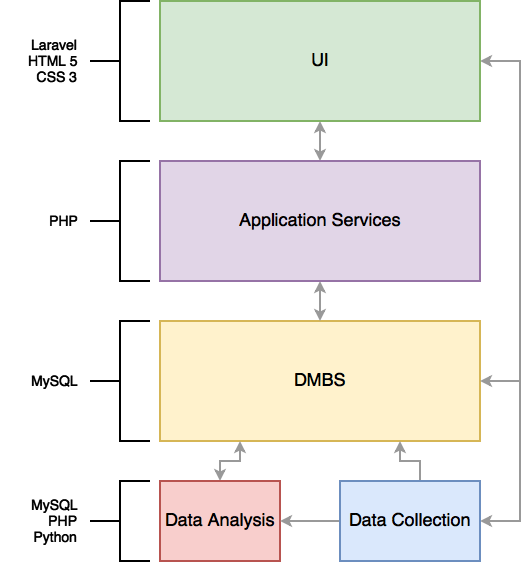
\includegraphics[width=0.5\textwidth]{Images/Design/LayerArchitecture}
  \caption{High Level System Design} \label{fig:LayerArchitecture} 
\end{figure}

\subsection{Overall System Architecture}
\begin{figure}[H]
  \centering
  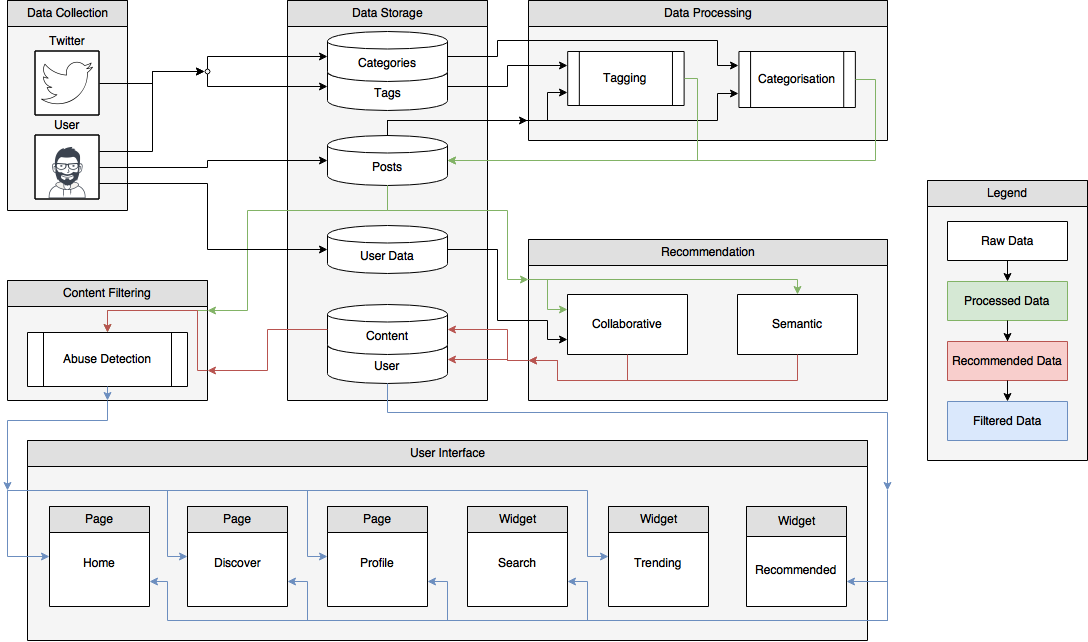
\includegraphics[width=1.0\textwidth]{Images/Design/SystemArchitecture}
  \caption{Proposed System Architecture Diagram} \label{fig:SystemArchitecture} 
\end{figure}

\section{Data Collection}

\subsection{Training Data}
Twitter, Kaggle, NLTK, etc.

\subsection{Template Data}


\subsection{User Authentication}
Manually

\section{Data Processing}
\subsection{Abuse Detection}
\subsection{Content Filtering}
\subsection{Recommendations}
Recommendations are a key component to Fidelis, and this section will look at the design of the algorithms for this purpose. Collaborative-based filtering was chosen as the filtering technique for recommendations. JustIfication for this is apparent in the technique itself; collaborative-filtering focuses on using the opinions of like-minded users, coupled with items rated by the user in the past. This sets up recommendations for success as they are much more likely to be greeted positively by the user. Given the nature of Fidelis as social network, resources in terms of previously rated items (through votes on posts) and like-minded users will be available in abundance to generate strong recommendations. It is important to provide the user with choice for how they would like to receive recommendations. To this end, the user will be provided with the option to choose how their recommendations should be provided. The following sections will look at the algorithm that will be used to generate recommendations for users, and will also discuss three different recommendation flavours that will be offered to the user, giving them final say on how their recommendations are generated. 

\subsubsection{User Recommendations}
\label{sec:user-recommendations}
Users are likely to interact with recommendations they receive on a daily basis. As such, algorithms generating recommendations should run on a daily basis. To generate recommendations, we must therefore first look at the number of recommendations already generated for each user. A user may choose not to interact with provided recommendations, so new recommendations should be made only when a user has approved or rejected their current recommendations. For each user, their item vector should be retrieved. The item vector will correspond to the features discussed in Chapter \ref{Chapter:Research}. The set of candidate recommendations for the user will be determined by what recommendation method they have chosen. Before checking for similarity between the user and the candidate recommendations, all users the user already follows, has blocked or has rejected as a recommendation should be removed from the candidate set. In the event that there are no candidate users, a default set of recommendations will be provided for the user. Using the retrieved collection of candidate recommendations, each user in this collection will be assessed to determine whether the similarity between them and the user is sufficiently large. Suitability between users will be determined using a threshold value. We are only interested in similarities that are at least as large as this value, as similarities less than the threshold value would mean that the two users in question are not similar. Only those users with a similarity greater than the threshold value should be provided as a recommendation. Similarity will be measured using cosine similarity. Cosine similarity is calculated using the following equation:
\begin{equation}
sim(\mathbf{A},\mathbf{B}) = \frac{\mathbf{A} \cdot \mathbf{B}}{\parallel\mathbf{A}\parallel \parallel\mathbf{B}\parallel} = = \frac{ \sum\limits_{i=1}^{n}{A_i  B_i} }{ \sqrt{\sum\limits_{i=1}^{n}{A_i^2}}  \sqrt{\sum\limits_{i=1}^{n}{B_i^2}} }
\label{eq:cos-similarity}
\end{equation}
Algorithm \ref{alg:user-recommendations} provides pseudocode for this process. Values for $similarityThreshold$ and $val$ should be set by the user.

\begin{algorithm}
\caption{User recommendations algorithm}
\label{alg:user-recommendations}
\begin{algorithmic}[1]
\State $similarityThreshold\gets 0.7$
\State $val\gets 5$
\ForAll{users $u$}
	\State $method\gets getRecommendationMethod(u)$
	\State $currentRecommendations\gets getNumberOfRecommendations(u)$
	\If{$currentRecommendations < val$}
		\State $uVector\gets getItemVector(u)$
		\If{$method = Friend$-$of$-$a$-$Friend$}
			\State $users\gets getFOFUsers(u)$
		\EndIf
		\If{$method = Explorer$}
			\State $users\gets getExplorerUsers(u)$
		\EndIf
		\If{$method = Hybrid$}
			\State $fof\gets getFOFUsers(u)$
			\State $explorer\gets getExplorerUsers(u)$
			\State $users\gets fof \cap explorers$
		\EndIf
		
		\State $uFollowing\gets getFollowing(u)$
		\State $uBlocked\gets getBlockedUsers(u)$
		\State $uRejected\gets getRejectedRecommendations(u)$
		\State $users = users \setminus uFollowing \setminus uBlocked \setminus uRejected$
		
		\If{$\left\vert{users}\right\vert = 0$}
			\State $getDefaultUsers$
		\Else
			\For{$v$ in $users$}
				\State $vVector\gets getItemVector(v)$
				\State $similarity\gets measureSimilarity(uVector, vVector)$
			
				\If{$similarity \geq similarityThreshold$}
					\State $storeRecommendation(v)$
				\EndIf
			\EndFor
		\EndIf
	\EndIf
\EndFor
\end{algorithmic}
\end{algorithm}

We will now look at each of the possible user sets for candidate recommendations. In particular, we will observe a general overview of the method for user selection and involves ourselves with a discussion on the method itself with regards to the wider system.

\begin{figure}[h]
	\centering
	\begin{subfigure}[b]{.3\linewidth}
		
\includegraphics[height=1.7in]{Images/Design/facebook}
		\caption{}
		\label{fig:fof-facebook}
	\end{subfigure}
	\begin{subfigure}[b]{.5\linewidth}
		
\includegraphics[width=1\linewidth]{Images/Design/linkedin}
		\caption{}
		\label{fig:fof-linkedin}
	\end{subfigure}
	\caption{Friend-of-a-Friend recommendations from (a) Facebook and (b) Twitter}
	\label{fig:fof}
\end{figure}

\paragraph{Friend-of-a-Friend Users}
With this method, candidate recommendations for a user $A$ are all users $C$ where $A$ follows $B$ and $B$ follows $C$. This method uses like-minded users for recommendations, and exploits the transitive nature of the ``following'' relationship. It is a popular technique used by numerous social networks, including Facebook (Figure \ref{fig:fof-facebook}) and Linkedin (Figure \ref{fig:fof-linkedin}). This option will allow the user to generate ``safer'' recommendations by using the idea that ``if $A$ trusts $B$, and $B$ trusts $C$, $A$ will most likely also trust $C$''. This is not always the case, but mostly holds true. It is important to give users this choice as it provides them more control over who enters their trust circle. Although one of the project aims is to burst opinion bubbles through exposure to different and trusted views, users must still be provided with this option. The function in Algorithm \ref{alg:fof-users} provides a procedure for retrieving ``$C$'' users. 

\begin{algorithm}
\caption{Function for getting Friend-of-a-Friend users}
\label{alg:fof-users}
\begin{algorithmic}[1]
\Function{getFOFUsers}{User u}
	\State $users = \emptyset$
	\State $uFollowing\gets getFollowing(u)$
	\For{$f$ in $uFollowing$}
		\State $fFollowing\gets getFollowing(f)$
		\State Add $fFollowing$ to $users$
	\EndFor
	\State \Return{$users$}		
\EndFunction
\end{algorithmic}
\end{algorithm}

\paragraph{Explorer Users}
Fidelis aims to expose users to opinions and users they may not initially interact with. Explorer users are chosen for exactly this reason. Candidate recommendations are found by finding users' favourite tags to post in and looking at other users who post in the same tag. This user collection method combines the users rated items and looks at like-minded users. By deviating from the users trust circle, we are more likely to generate recommendations that will broaden user opinions by finding other users who care about the same topics, but will naturally hold different views on them. This method seeks to expand a users trust circle beyond current opinions held by them. The function in Algorithm \ref{alg:explorer-users} shows the procedure for collecting Explorer users. $N$ is used to determine the number of tags that will be searched for candidate recommendations. The function in Algorithm \ref{alg:explorer-users} shows this procedure.

\begin{algorithm}
\caption{Function for getting Explorer users}
\label{alg:explorer-users}
\begin{algorithmic}[1]
\Function{getExplorerUsers}{User u}
	\State $threshold\gets 75$
	\State $users\gets \emptyset$
	\State Get $N$ top tags $u$ posts in
	\For{$tag t = 1$ to $N$}
		\State Get all users $v$ posting in $t$
		\If{$reputationOf(v) >= threshold$}
			\State Add $v$ to $users$
		\EndIf
	\EndFor
	\State \Return{$users$}
\EndFunction
\end{algorithmic}
\end{algorithm}

\paragraph{Hybrid Users}
Using this method aims to find the middle ground between the two aforementioned techniques. The intersection between Explorer and Friend-of-a-Friend users, as shown in Figure \ref{fig:hybrid}, is returned as the set of candidate recommendations. 

\begin{figure}
\centering
\begin{tikzpicture}[
    thick]
    \draw [fill=cyan, fill opacity=0.5, name path=c1] (0,0) circle (2cm);
    \draw [fill=orange, fill opacity=0.5, name path=c2] (3,-1) circle (2.5cm);
    \draw (0,0) ++(120:2cm) -- ++(120:2.2cm) node [fill=white,inner sep=5pt](a){Friend-of-a-Friend};
    \draw (3, -1) ++(30:2.5cm) -- ++(30:2.6cm) node [fill=white,inner sep=5pt](b){Explorer};
    \path [name intersections={of=c1 and c2,by=cs}];
    \draw (cs) -- ++(.5,1) node [fill=white,inner sep=5pt](c){Hybrid};
\end{tikzpicture}
\caption{Hybrid user selection}
\label{fig:hybrid}
\end{figure}

\paragraph{Default Recommendations}
If all aforementioned methods fail to return a set of candidate recommendations, the system should revert to default candidate recommendations. This method will return either the $N$ most popular or reputable users on Fidelis. The function in Algorithm \ref{alg:default-users} shows this procedure for most popular users, but the same procedure can be re-used for getting the most reputable users.

\begin{algorithm}
\caption{Function for getting default users}
\label{alg:default-users}
\begin{algorithmic}[1]
\Function{getDefaultUsers}{User u}
	\State $users\gets \emptyset$
	\State $users\gets getMostPopularUsers$
	\State $users\gets sortDescending(users)$
	\State \Return{$N$ top users from $users$}
\EndFunction
\end{algorithmic}
\end{algorithm}

\subsubsection{Content Recommendations}
\label{sec:content-recommendations}
Similarly to user recommendations, users will interact with content recommendations made for them daily and so new content recommendations should be generated for them daily also. Again, before any new recommendations are made we must look at how many recommendations the user currently has. By doing this, we limit any unnecessary computation. In the case of content recommendations, user item vectors will not be used. It was instead decided to use the reputation of a given post, rather than the similarity between the user recommendations are being generated for and the author of the post. The justification behind this is that user recommendations should focus on locating like-minded users, whereas content recommendations should avoid this to diversify the content made available to users. Providing recommendations in this manner again emphasises the desire for Fidelis to break the constraints of the ``echo chamber effect'' currently restricting most social media platforms. By letting the user pick a reputation threshold for recommendations generated for them, we can ensure that users trust their recommendations and can confidently interact with them knowing they are trustworthy. Algorithm \ref{alg:content-recommendations} provides the pseudocode for the procedure described above. 

\begin{algorithm}
\caption{Content recommendations algorithm}
\label{alg:content-recommendations}
\begin{algorithmic}[1]
\State $val\gets 5$
\State $reputationThreshold\gets 0.7$
\ForAll{users $u$}
	\State $method\gets getRecommendationMethod(u)$
	\State $currentRecommendations\gets getNumberOfRecommendations(u)$
	\If{$currentRecommendations < val$}
		\If{$method = Friend$-$of$-$a$-$Friend$}
			\State $posts\gets getFOFPosts(u)$
		\EndIf
		\If{$method = Explorer$}
			\State $posts\gets getExplorerPosts(u)$
		\EndIf
		\If{$method = Hybrid$}
			\State $fof\gets getFOFPosts(u)$
			\State $explorer\gets getExplorerPosts(u)$
			\State $posts\gets fof \cap explorers$
		\EndIf
		
		\State $uVoted\gets getVotedPosts(u)$
		\State $uBlocked\gets getBlockedPosts(u)$
		\State $posts = posts \setminus uVoted \setminus uBlocked$
		
		\If{$\left\vert{posts}\right\vert = 0$}
			\State $getDefaultContent$
		\Else
			\For{$p$ in $posts$}
				\If{$getReputation(p) \geq reputationThreshold$}
					\State $storeRecommendation(p)$
				\EndIf
			\EndFor
		\EndIf
	\EndIf
\EndFor
\end{algorithmic}
\end{algorithm}

We will again look at how each of the four recommendation techniques will generate candidate post sets. By providing the user with different ways recommendations can be generated for them will again ensure that users are in control of content they will interact with. 

\paragraph{Friend-of-a-Friend content} Candidate recommendations using this method will build on the follows relationship mentioned earlier in Chapter \ref{sec:user-recommendations} by retrieving the posts from Friend-of-a-Friend users. Getting content in this manner will provide users with a selection of posts that are likely to agree with their own sentiments. 

\begin{algorithm}
\caption{Function for getting Friend-of-a-Friend content}
\label{alg:fof-content}
\begin{algorithmic}[1]
\Function{getFOFUsers}{User u}
	\State $posts\gets \emptyset$
	\State $uFollowing\gets getFollowing(u)$
	\For{$f$ in $uFollowing$}
		\State $fFollowing\gets getFollowing(f)$
		\For{$g$ in $fFollowing$}
			\State $gPosts\gets getPosts(g)$
			\State Add $gPosts$ to $posts$
		\EndFor  
	\EndFor
	\State \Return{$posts$}		
\EndFunction
\end{algorithmic}
\end{algorithm}

\paragraph{Explorer content} Explorer content recommendations stress the idea previously mentioned about removing the constraints of the ``echo chamber effect''. By considering other users who post in the same categories as the user recommendations are being generated for, we only consider posts that the user will be interested in. Without considering the similarity between the authors of these posts and the user themselves, we increase the likelihood of exposing users to content they would not normally interact with.

\begin{algorithm}
\caption{Function for getting Explorer content}
\label{alg:explorer-content}
\begin{algorithmic}[1]
\Function{getExplorerPosts}{User u}
	\State $posts\gets \emptyset$
	\State $users\gets getExplorerUsers(u)$
	\For{$u$ in $users$}
		\State $uPosts\gets getPosts(u)$
		\State Add $uPosts$ to $posts$
	\EndFor
	\State \Return{$posts$}
\EndFunction
\end{algorithmic}
\end{algorithm}

\paragraph{Hybrid content} Using this method aims to find the middle ground between the two aforementioned techniques. We take a similar approach as to before and return the intersection between Explorer and Friend-of-a-Friend content as the set of candidate recommendations.

\paragraph{Default content} Default content recommendations will return the $N$ most popular or reputable posts made on Fidelis. . The function in Algorithm \ref{alg:default-content} shows the procedure for retrieving the most popular posts, but the same procedure can be re-used for getting the most reputable posts.

\begin{algorithm}
\caption{Function for getting default content}
\label{alg:default-content}
\begin{algorithmic}[1]
\Function{getDefaultContent}{}
	\State $posts\gets \emptyset$
	\State $posts\gets getMostPopularPosts$
	\State $posts\gets sortDescending(posts)$
	\State \Return{$N$ top posts from $posts$}
\EndFunction
\end{algorithmic}
\end{algorithm}

\subsection{Reputation Scoring}

\section{Database}

\section{User Interface}

\section{Responsive Design}
\chapter{Implementation}
\label{Chapter:Implementation}
Having provided detail on the design stage of the project, this chapter of the report begins to look moving from concepts to implementation. The web application being built will provide a way of delivering Fidelis to multiple users across multiple devices rather than creating a separate application tailored to each platform. The following sections will look at the technologies used to implement the application, along with detailed information on algorithm and UI implementation.

\section{Technologies}
Building Fidelis required collating a number of technologies. The technologies used for implementation can be categorised into storage, processing and visualisation technologies, each of which are discussed below.

\subsection{Storage}
MySQL is an open source database management system used for managing data held in a relational database management system \cite{MySQL:Home}. It is the world's most popular open source database, being used by some of the largest and fastest-growing organisations including Facebook, Google and Adobe. The reasons behind the use of MySQL database are vast but the key factor is the ease with which a MySQL database can be setup and migrated. MySQL databases have existed for many years which has led to gradual improvements over time, and as a result of these improvements MySQL databases now guarantee stability, scalability and security \cite{MySQL:Why}. The longevity of MySQL database systems is another appealing aspect, and has meant that a wide range of third-party party tools are available to the developer for working with and processing the data. 

\subsection{Processing}
Majority of the data processing will be done using PHP. All PHP scripts are executed on the server which may produce output that can be presented to the user. The language is used by millions of websites and has for some time been  a popular scripting language for dynamic web development. This wide adoption of the PHP scripting language has allowed extensive libraries and frameworks to be made available and used for rapid development of web applications. One such framework, Laravel, will be used to implement the MVC approach discussed in Chapter \ref{Chapter:Research}. PHP has shown to be scalable as it is powerful enough to be at the core of the biggest blogging system on the web, known as WordPress, but at the same time it is deep enough to run the largest social network, Facebook\cite{W3Schools:PHP_Intro, Wiki:WordPress, Fastcompany:Facebook_PHP}. This means that in the future if the system is to grow large enough, it can easily be scaled as done so over time by the aforementioned examples. 

In addition to PHP, JavaScript will be used for some client-side data processing along with SQL which will be used to process data from the database before it is retrieved. Python will be used to process user data needed for content-filtering, abuse detection, recommendations and reputation scoring. Like PHP, Python is also executed on the server-side, reducing the amount of processing and computation required on the client-side. Python was chosen not only for its popularity, but again like PHP it provides an extensive range of libraries that can be used during development. Examples of these include Scikit-Learn \cite{scikit:home}, which provides a number of data mining and analysis tools, and \emph{NumPy} and \emph{pandas}, which are useful for data manipulation.

It was mentioned in Chapter \ref{Chapter:Design} that it would not be feasible to run the data processing algorithms in real-time, and as such these would need to be scheduled to run at set intervals. Cron is a unix- system utility that is used to execute tasks at designated times \cite{Ubuntu:Cron}. Tasks that are scheduled for execution are contained in a \textit{crontab} file. Entries in the file appear as:
\begin{lstlisting}[language=bash]
* * * * * cmd/to/run
\end{lstlisting}

\noindent Each asterix represents a time-and-date field, and from left to right these correspond to minute, hour, day, month and weekday \cite{Ubuntu:Cron}. 

Laravel contains a task scheduler which simplifies the process of executing tasks at a given interval. With the scheduler, only the following entry needs to be added to the \textit{crontab} file:

\begin{lstlisting}[language=bash]
* * * * * php /path-to-your-project/artisan schedule:run >> /dev/null 2>&1
\end{lstlisting}

\noindent This entry calls the Laravel task scheduler every minute \cite{Laravel:Scheduling}. Laravel's task scheduler provides a number of schedule frequency options, including daily, weekly or even as a custom cron entry \cite{Laravel:Scheduling}. Tasks can be added to the \texttt{schedule()} method in \textit{app/Console/Kernel}. In the method, it is possible to schedule Artisan commands, which can be made by the user, or OS commands. Figure \ref{fig:FidelisSchedule} shows the tasks scheduled to run daily at midnight.

\begin{figure}[H]
\centering
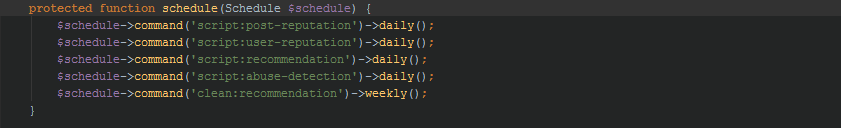
\includegraphics[height=1in]{Images/Implementation/FidelisSchedule}
\caption{Scheduled tasks for Fidelis}
\label{fig:FidelisSchedule}
\end{figure}


\subsection{Visualisation}
HTML is coupled with CSS to define page structure, and design the components on the page \cite{W3:HTML5, W3:CSS}. In addition to this, the Laravel blade engine is being used to make the generation of pages easier by splitting content up into views that can be extended by or rendered inside other views \cite{Laravel:Blade}. This encourages good practices by abstracting the system and enforcing modularity throughout. Using the blade enginge supported the idea of using component-driven design, discussed in Chapter \ref{Chapter:ProjectManagement}. Building views in a modular fashion enables development in the future to easily integrate new components and replace master views seamlessly to change the overall system appearance. Bootstrap is also used as an additional framework to make the pages more dynamic by providing visual interaction.

\subsection{Installation and Setup}
Many of the technologies being employed are not included by default on an ordinary machine. Thus, before development could be initiated, it was necessary to install and configure the required technologies. This section details the configuration process for the technologies used, along with any prerequisites for them.

\subsubsection{Initial Setup}
An Apache web server capable of interpreting PHP and rendering web pages was required for development. In addition to this, an SQL server was need to host the MySQL database. XAMPP, which provides an SQL and web server, was the solution chosen to handle both these cases. Both servers are automatically configured by the XAMPP package upon installation and are immediately ready to use out of the box. XAMPP provides an easy-to-use control panel from which servers can be started, and accessing through \textit{http://localhost/}. Any files can them be placed inside the \textit{htdocs} folder, created during the installation process.

\subsubsection{IDE and Laravel}
The Laravel framework was used to build Fidelis, but it is not readily available to download as an archive. Instead, composer - a package manager, was used for the installation of the framework. Using composer, new projects can be created using the \textit{laraval new project-name} command. Executing this command creates a new \textit{project-name} directory with all the necessary files and project dependencies. Updates and additional packages may be installed using composer and the included \textit{packages.json} file.

The PHPStorm IDE, developed by JetBrains, was used throughout the project for all web-related development. PHPStorm is a dedicated PHP IDE, and has the capability to include plugins providing features that enable the use of frameworks like Laravel. The IDE also makes available a set of tools that made writing code more efficient and effective. 

\section{Routing and Middleware}
Laravel allows the developer to define custom routes in contrast to the normal approach where routes are determined by page URI. In addition to this, Laravel enables developers to use middleware for filtering HTTP requests. Both of these approaches, used for implementing user friendly URLs and security, are discussed in this section.

\subsection{Routes}
Application routes are defined inside the \textit{routes.php} file, which is automatically loaded by the framework \cite{Laravel:Routing}. The easiest way to define a route in Laravel is by passing a URI and a closure which is executed when the URI is hit. A closure can be thought as a handler for what should occur when a URI is hit. However, this approach limits the functionality of the application and instead we can pass the name of a controller followed by the name of the method which is to be called if a URI is hit. Routes can be grouped together if they share common features of functionality. For example, all the routes are contained within the default 'web' middleware group, which provides access to session state and CSRF protection \cite{Laravel:Routing}.

\begin{figure}[H]
	\centering
	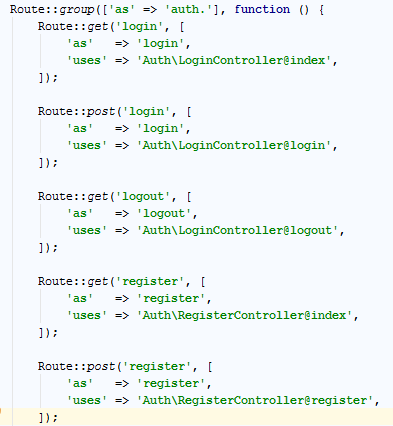
\includegraphics[height=2.5in]{Images/Implementation/LaravelRouting}
	\caption{A subset of the routes fefined in the authentication} \label{fig:Routes}
\end{figure}

Figure \ref{fig:Routes} shows the code which defines all the routes regarding the different user authentication components. The routes are grouped together with a prefix using the \emph{'as'} parameter. This adds the 'auth::' prefix to the name of each route. For example, using \emph{route('auth::login')} will generate the URL pointing to the login page for user authentication. In addition to this, parameters can be included with the request for a route request, allowing for more flexible URLs. Included paramemters are passed to the relevant controller for the route. 

Routing with Laravel allows requests to be restricted to a certain type. With this, we can achieve security by limiting the type of HTTP request a route will accept. Laravel provides get, post, put, patch, and delete options for each route. A route defined using \emph{route::post} may only be accessed if the user posts form data to the URL. It is possible to bind a route to multiple request types such as get and post or even all request types but this is generally not recommended.

\subsection{Middleware}
HTTP middleware provides a convenient mechanism for filtering HTTP requests entering your application \cite{Laravel:Middleware}. Middleware is generally executed before a page is loaded in order to assess whether the user can access the page. It is possible to associate a page with multiple middlewares, and this can be thought of as a chain of middleware - requirements being passed from a previous middleware triggers a call to the next one. A middleware can be assigned to a route, method, controller or even a group of middleware.

It is possible to create custom middleware using the Artisan utility. The \textit{php artisan make:middleware Demo} command will generate a middleware called Demo. The image in figure \ref{fig:MiddlewareTemplate} shows the template that is generated by the Artisan utility. The commented block on line 17 can be replaced with a check, which if passed allows the next middleware to be activated but if failed returns an alternative action to be executed. Middleware was used in Fidelis to achieve several trivial tasks in the application, each of which are discussed in the relevant sections through the rest of this chapter.

\begin{figure}[H]
	\centering
	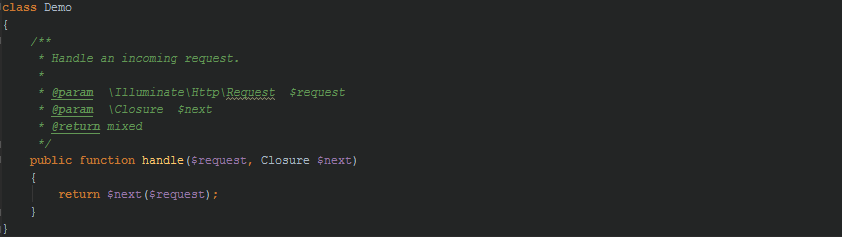
\includegraphics[height=2in]{Images/Implementation/MiddlewareTemplate}
	\caption{Middleware Template Generated by the Artisan Utility} \label{fig:MiddlewareTemplate}
\end{figure}

\section{Data Collection}

\section{Data Processing}
As mentioned earlier, Python was chosen for data processing. Python has an established data analysis community, and as such provides a rich assortment of open-source libraries that can be used. With a such a community, documentation was abundant and meant that the implementation of the designs discussed in Chapter \ref{Chapter:Design} were accelerated greatly. Not only this, but existing solutions for problems encountered during development were 
available, which again sped up the implementation process. 

\subsection{Abuse Detection}
\subsection{Content Filtering}
\subsection{Content Recommendation}
Content recommendations are generated from a single python script. It was decided to go with a single script as certain techniques are shared between user and post recommendations. The script is modularised by using functions that enable code blocks to be re-used. Python list comprehension provides a succinct way to generate lists \cite{Python:ListComprehension}, and this syntax is used throughout implementation.

Before recommendations can be made, a database connection is established using the mysql.connector library, ``a Python driver for communicating with MySQL servers'' \cite{MySQL:MySQLConnector}. This library contains a number of useful functions for database interactions. Recommendation generation only occurs if the attempt to connect to the database is successful, otherwise an error message is logged. This prevents erroneous system behaviour. To begin recommendations, all users are first retrieved from the database. To tailor recommendations to a specific user, user settings for how they want their recommendations to be generated are retrieved. Default settings are set for new users but these can be changed on the settings page. The settings retrieved are for recommendation preference (FOF, Explorer or Hybrid recommendations), the number of recommendations to generate, recommendation threshold (for vector similarity) and recommendation reputation. Figure \ref{fig:RecommendationSettings} shows how user settings are retrieved.


\begin{figure}[H]
\centering
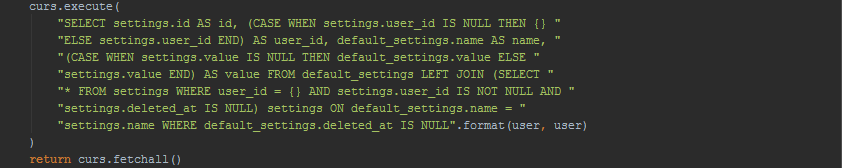
\includegraphics[height=2in]{Images/Implementation/RecommendationSettings}
\caption{Function that executes query for retrieving user settings}
\label{fig:RecommendationSettings}
\end{figure}

\noindent Letting the use have control over this settings will allow them to fine-tune how they want to receive recommendations. The next two sections will look at how user and post recommendations are generated.

Recommendations are generated using either FOF, Explorer or Hybrid users. The technique chosen for generation is dependent on the preference set by the user. To begin with, a query retrieving a count of the number of user recommendations already generated for the user is retrieved. New recommendations are only made if this count is less than the number of recommendations specified by the user. We will now look at how each of these techniques are implemented. Processes will be discussed for an individual user, who we will refer to as the recommendee, but each is repeated for all users stored in the database.

\subsubsection{Friend-of-a-Friend Recommendations}
FOF candidate recommendations are retrieved by first getting all users followed by the recommendee. These users are looped through, and for each of them the users they follow are collected and appended to a list. The recommendee is excluded from this list. Once this list has been generated, it is flattened to become a single list, which we will refer to as the \textit{fof\_users} list.

\paragraph{User} From this list, FOF user recommendations are chosen by converting the list to a Counter object and picking the most common elements. The counter object was used for this purpose as it enables quick tallying \cite{Python:Counter} the \texttt{most\_common()} method on Counter objects accepts a parameter value for the number of common elements to be returned. This ensures that only the number of required recommendations for the recommendee are returned. Use of the Counter object is given below:

\begin{lstlisting}[language=python]
fof_users = Counter(fof_users).most_common(num_recommendations)
\end{lstlisting}

Reasoning for not using cosine similarity between candidate recommendations and the recommendee are given in Chapter \ref{Chapter:Design}.

\paragraph{Post} Using the same technique for post recommendations, the users in the \textit{fof\_users} list are looped through, retrieving the posts made by each of the  users. For a post to suffice as a candidate recommendation for the recommendee, its reputation is compared with the reputation threshold set by the recommendee. If the reputation of the post exceeds the threshold, it is returned as one of the posts in the list of recommendations for the recommendee.

\begin{figure}[H]
\centering
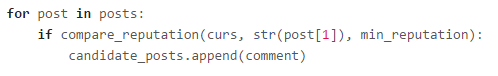
\includegraphics[height=0.7in]{Images/Implementation/FOFPostReputation}
\caption{Code for assessing the reputation of a candidate post recommendation}
\label{fig:FOFPostReputation}
\end{figure} 

\noindent Figure \ref{fig:FOFPostReputation} shows the process for comparing the reputation of a candidate post recommendation with the minimum reputation set by the user. Performing this check ensures again that recommendations being made are tailored to the recommendee's preferences.

\subsubsection{Explorer Recommendations}
Explorer recommendations make use of the recommendee's `tag count vector', which is a vector representing the number of posts the recommendee has made in each of the available tags. The vector is generated by first creating a zero-filled list which has a length equal to the number of tags currently stored. Each entry in the list is a (TagID, Count) tuple. This list, which we shall refer to as the recommendee\_vector is then sorted to determine the recommendee's favourite tags to post in. Candidate recommendations are retrieved from these tags. Currently, there is no cap on the number of tags looked at, but a cap on the number of ``favourite tags'' can be set once the system grows beyond what is considered small. The recommendee's favourite tags are looped through, retrieving other users posting in the same tag. This is shown in Figure \ref{fig:ExplorerFavouriteTags}.

\begin{figure}[H]
\centering
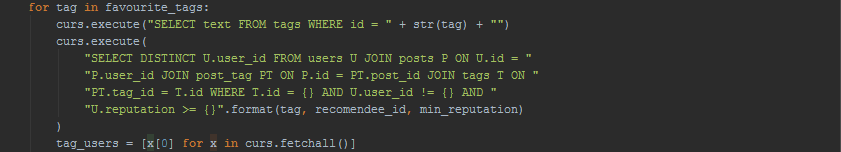
\includegraphics[height=2in]{Images/Implementation/ExplorerFavouriteTags}
\caption{Code for retrieving users who post in the recommendee's preferred tags}
\label{fig:ExplorerFavouriteTags}
\end{figure}

\paragraph{User} Explorer user recommendations are assessed based on the similarity between a tag user (user also posting in one of the recommendee's preferred tags) and the recommendee. Similarity is measured using cosine similarity. SciPy provides a number of distance computation functions, one of which the cosine distance. This is used to measure the distance between the vector generated for the tag user and the recommendee's vector. To get similarity from this, the result of this measurement is subtracted from one.

\begin{figure}[H]
\centering
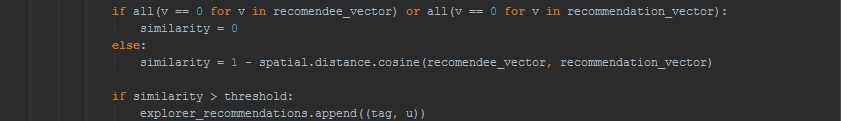
\includegraphics[height=2in]{Images/Implementation/ExplorerSimilarity}
\caption{Measuring similarity between users for Explorer recommendations}
\label{fig:ExplorerSimilarity}
\end{figure}

\noindent In Figure \ref{fig:ExplorerSimilarity}, we see that we need to account for a user vector containing all zeros. This is possible for new or existing users who have made no posts. To account for this, similarity is only measured if neither of the two user vectors contain only zeros. Once similarity is measured, it is compared with the threshold for similarity set by the user. Only users with a similarity that exceeds this threshold are given as recommendations. In the figure we can see again that recommendations are saved as (TagID, Before the set of user recommendations is returned, its length is compared with the number of recommendations needed to provide only the required number of recommendations. 

\paragraph{Post} Similarly to post recommendations generated using the FOF technique, posts made by each of the tag users are retrieved. Only those exceeding the reputation set by the recommendee are given as recommendations. Akin to user recommendations, only the number of required recommendations are returned.

\subsubsection{Hybrid Recommendations}
Hybrid recommendations are generated by finding the intersection between the recommendations made using the FOF and Explorer recommendation methods. The Python Standard Library provides a \textit{sets} module, which can create a set of unordered, unique elements from a list \cite{Python:Sets}. Using this module, it is possible to convert the lists returned from each of the recommendation methods to sets and find the intersection between the two. We can see this in Figure \ref{fig:HybridRecommendations}.

\begin{figure}[H]
\centering
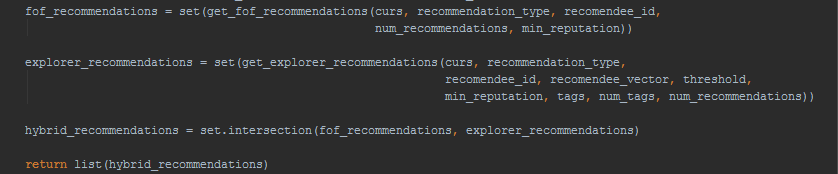
\includegraphics[height=1.5in]{Images/Implementation/HybridRecommendations}
\caption{Generation of hybrid recommendations}
\label{fig:HybridRecommendations}
\end{figure}

\subsubsection{Default Recommendations}
In the event that all previous methods for generating recommendations fail, the script reverts to a default method that will generate generic recommendations for the recommendee. 

\paragraph{User} Generic user recommendations will consist of users with the highest reputation in the system. To further filter this, only users with a reputation greater than the minimum reputation set by the user are returned.

\begin{figure}[H]
\centering
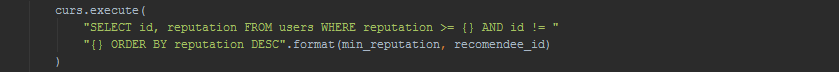
\includegraphics[height=0.7in]{Images/Implementation/DefaultUsers}
\caption{Query for selecting most reputable users}
\label{fig:DefaultUsers}
\end{figure}

\paragraph{Post}
Similarly to users, default post recommendations are made based off the most reputable posts in the system.

\begin{figure}[H]
\centering
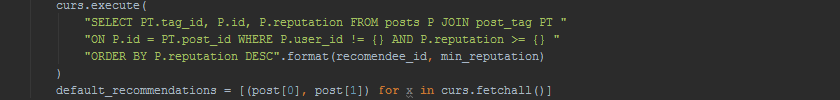
\includegraphics[height=1in]{Images/Implementation/DefaultPosts}
\caption{Query for selecting most reputable posts}
\label{fig:DefaultPosts}
\end{figure}

\subsubsection{Cleaning and Saving Recommendations}
Once recommendations have been generated, they need to be cleaned. The first step in cleaning involves removing any recommendations the user currently has and has not responded to. In addition to this, cleaning user recommendations consists of:
\begin{itemize}
\item Removing blocked users
\item Removing users the recommendee already follows
\item Removing the recommendee themselves
\end{itemize}

\noindent Cleaning post recommendations consists of:
\begin{itemize}
\item Removing posts made by users the recommendee has blocked
\item Removing posts the recommendee has voted on and therefore has already seen
\end{itemize}

In the case of cleaning post recommendations, posts made by the recommendee are not removed as all queries involving candidate post recommendations omit posts made by the recommendee.

Once recommendations have been cleaned, new recommendations are inserted into the relevant table. After storing the recommendations, changes made to the database must be commited using the \texttt{commit()} function on the connection object.

\subsection{Reputation Scoring}

\section{Database}
The database is at the core of the application and thus care must be taken when setting up and configuring the database. A range of tools, provided by Laravel, were employed for configuring and interacting with the database. Details of the configuration and setup are discussed in detail.

\subsection{Configuration}
Database interactions occur through models, the query builder, schema builder and migrations provided as part of the Laravel framework. Settings inside the projects' configuration file must be tweaked in order for these components to function correctly. These settings allow the developer to change the connection, authentication and driver details for the application. In this project setup the PDO driver was used to connect to the database. Figure \ref{fig:DatabaseConfig} shows some of the settings that may be tuned in the configuration file.

\begin{figure}[H]
	\centering
	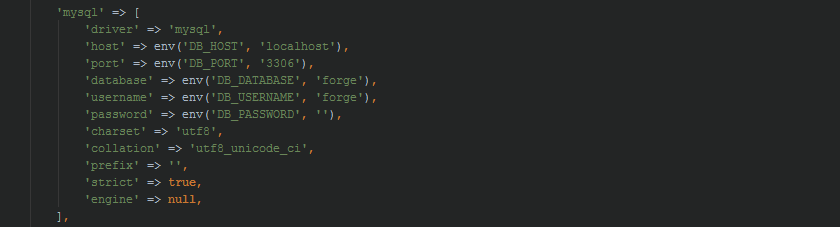
\includegraphics[height=2.3in]{Images/Implementation/MySQLConfig}
	\caption{Database Configuration for MySQL Databases} \label{fig:DatabaseConfig}
\end{figure}

\subsection{Migrations}
Migrations in Laravel are used to build database tables, and act as a database version control system, ``allowing a team to easily modify and share the application's database schema'' \cite{Laravel:Migrations}. The use of migrations not only allows for the database to be replicated anywhere the system is installed with ease but also simplifies the process of updating an existing table during the development process.  To create a migration, the \emph{make:migration}command provided by the Laravel Artisan utility is used. This command generates an empty template for a specified table. When creating a new table, the \emph{--create} argument is used whereas the \emph{--table} argument is used for modifying an existing table. The generated template contains an \emph{up} method, used for adding new columns and index, and a \emph{down} method which reverses the changes produced by the \emph{up} method. Migrations are typically paired with Laravel's schema builder to easily build your application's database schema \cite{Laravel:Migrations}. The schema builder can be used to define the schema for the table using calls to PHP functions. Once the schema has been populated, the \emph{migrate} command can be used to run the migration and update the database. In the case of an error the users can revert to a previous version of the database using the \emph{migrate:rollback} command. It is always encouraged that major changes, such as adding new columns and adding indexes, are introduced using new migrations rather than rolling back and updating existing migrations. All database tables were created using Laravel migrations and are available in the code.

\begin{figure}[H]
	\centering
	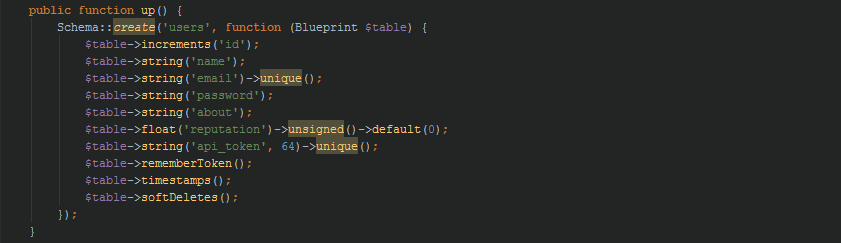
\includegraphics[height=2in]{Images/Implementation/UserMigration}
	\caption{Migration for creating Users table} \label{fig:UserMigration}
\end{figure}

Figure \ref{fig:UserMigration} shows the migration for the users table, which is used to store user information. The migration in the figure is not the final schema, and rather is the schema used during development. Additional migrations were used to add and modify columns in the table. As visible in the image, the schema builder can be used in the up method to define the structure of the table. Each migration schema contains an \emph{id} field, generated by calling the \emph{increments} method, and the \emph{created\_at} and \emph{updated\_at} timestamps, generated by calling the \emph{timestamps} method, by default. The \emph{increments} method is used for assigning an auto incrementing primary key, discussed later in the report, used for associating record through relationships. A \emph{deleted\_at} timestamp was added to all tables by calling the \emph{softDeletes} method. A range of other method such as \emph{string} and \emph{integer} can be used for creating more attributes. A full list of operations is available in the Laravel documentation \cite{Laravel:Migrations}. 

\subsection{Functional Dependencies and Constraints}
Majority of the foreign key constraints used in the database were setup with cascade delete and cascade update. This means that if a row in the referenced entity is removed or updated then any rows in the referencing entity which correspond to it are also updated or deleted \cite{TechOnTheNet:Cascading}. Some of the constraints followed the schema-bound dependencies by using the restrict keyword which prevents changes in the referenced entity if corresponding rows exist in the referencing entity. The use of all these techniques ensures that data is always kept consistent and no redundant data is introduced into the system.

\subsection{Security}
Security is of the upmost importance when it comes to a database which contains sensitive or personal information about individuals. For this reason, several measures should be taken into consideration to protect the database and the data in it from unauthorised access. The security threats and approaches taken to protect against them are discussed below.

\subsubsection{Access}
The first step to protecting the data is controlling who has access to the database and who is authorised to do what. This was achieved by creating separate SQL user accounts with different privileges. The database was then protected using a password to prevent any unauthorised access and only authorised users with a username and password would be able to access the database. Furthermore, each user was restricted so that the database would accept connections from the user if they were from a specified IP address. This meant that database connections could be restricted to just the web server and any users attempting to connect to the database from other machines would be denied access. When connecting to the database through PHP, root account was used for development purposes to prevent any restrictions but a separate account was used for production which was unable to modify the schema but could still query or modify the data.

\subsubsection{SQL Injection}
``SQL injection is a technique where malicious users can inject SQL commands into an SQL statement, via web page input'' \cite{W3Schools:SQL_Injection}. According to a report on 5,500 companies and 15,000 websites, almost half of these were vulnerable to serious security threats by XSS or SQL injection \cite{FirstPost:Vulnerabilities}. SQL injection can lead to all the data held in a database being made available. This is a serious threat as some of the data can be used to identify individuals and measures should be introduced to protect against this. One way to prevent SQL injection is by escaping all user input to prevent users from executing malicious queries. This is not a full fix for the issue as users can still enter data that can cause the system to malfunction. The alternative fix for this was using prepared queries which executes the query with placeholders and then binds the values later to retrieve the records. This method escapes SQL injection and prevents any unauthorised interaction with the database.

\subsection{Querying}
Laravel makes running queries extremely simple using either raw SQL statements, the fluent query builder, or the Eloquent Object-Relational Mapping (ORM) \cite{Laravel:Database}. For most part the Eloquent ORM approach was used to retrieve the result from the database but the approaches have been used in rare cases. All three approaches are outlined below.

\paragraph{Raw SQL}
With Laravel, raw SQL statements can be executed using the provided built-in classes. This removes the need to open a database connection, create SQL statements and bind parameters to these statements as this is all done automatically. For example, as shown in the example below, the user can run an SQL query to retrieve a user with a specific ID of 1 just by using the \emph{DB::select} method:

\begin{lstlisting}[language=php]
$users = DB::select('SELECT * FROM users WHERE id = ?', [1]);
\end{lstlisting}

\noindent The above query will return an array of objects modelling the user entity in the database. Using this array, it is possible to loop through the array and access the properties of each user as \emph{\$user-$>$property}, where property may be any attribute such as username or email.

\paragraph{Query Builder}
The database query builder provides a convenient, fluent, and easy-to-use interface for creating and executing database queries \cite{Laravel:QueryBuilder}. The query builder can perform most operations supported by the database driver. One of the main advantages of using the query builder is that it uses PDO parameter bindings to prevent SQL injections, which means there is no need to sanitise user input. Using the query builder, one could retrieve the user with ID 1 by executing the following statement:

\begin{lstlisting}[language=php]
$user = DB::table('users')->where('id', 1)->first();
\end{lstlisting}

\noindent The above query would fetch the result where the user ID matches the provided parameter and retrieve the first result. Once again, the result is returned as an object modelling the user entity and the properties can be accessed again as \emph{\$user-$>$property}.

\paragraph{Eloquent Object-Relational Mapping}
The Eloquent ORM included with Laravel provides an simple and elegant active record implementation for working with the database \cite{Laravel:Eloquent}. "Object-relational mapping (ORM) is a mechanism that makes it possible to address, access and manipulate objects without having to consider how those objects relate to their data sources" \cite{TechTarget:ORM}. Each database table has a corresponding "model" associated with it that is used database interactions and more specifically the table corresponding to a given model. Models allow the developer to query, insert, update, and delete records in the corresponding table as well as more complex operations such as joining tables. When querying the database using a model, Eloquent automatically instantiates and maps a model for each row in the result allowing the developer to utilise the models behaviour.

\begin{lstlisting}[language=bash]
$ php artisan make:model Models/User
\end{lstlisting}

\noindent Creating a model is made simple again thanks to the Artisan utility. The command above will generate a User model in the \emph{app/Models} directory. Each Eloquent models extends the \emph{Illuminate/Database/Eloquent/Model} class which utilises the query builder for all interactions \cite{Laravel:Eloquent}. By default, Eloquent assumes that each table has a primary key field named \emph{id} and the \emph{created\_at} and \emph{updated\_at} timestamps but these can all be changed by toggling optional properties in the model. In order to use a model, the developer simply needs to import the model in the controller where it will be used. The user can simple execute the following command in order to retrieve the user with ID=1.

\begin{lstlisting}[language=php]
$user = User::find(1);
\end{lstlisting}

\noindent The line of code above will return the \emph{User} model. It is again possible to access the model properties as \emph{\$user-$>$property}. The main change to be noticed here is that the user can actually update the properties and save the changes made by executing the following: \emph{\$user-$>$save()} \cite{Laravel:Eloquent}.  The image in figure \ref{fig:UserModel} shows the code for the \emph{User} model. As visible in the image, it is possible to add custom methods to the model which may be called when the model is returned as a result.

\begin{figure}[H]
	\centering
	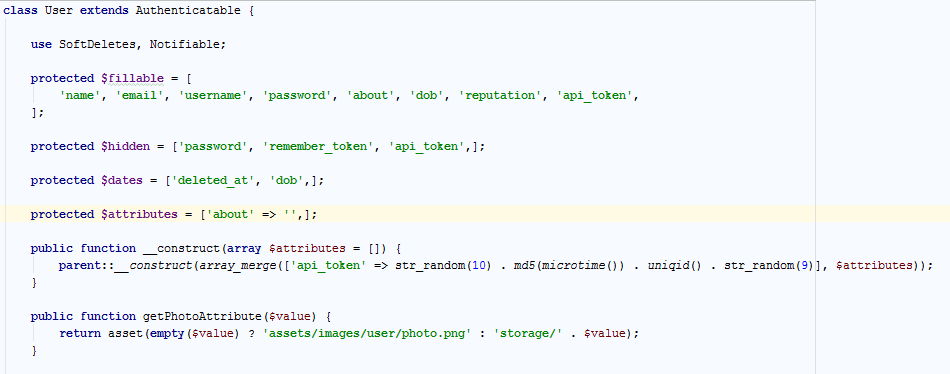
\includegraphics[width=1.0\textwidth]{Images/Implementation/UserModel}
	\caption{Users Eloquent ORM model} \label{fig:UserModel}
\end{figure}

\section{User Interface}
\subsection{Navigation}
\subsection{Authentication}
\subsubsection{Registration}
\subsubsection{Login}
\subsubsection{Recover Account}
\subsubsection{Authorised Access}
\subsection{Home}
\subsection{Discover}
\subsection{Notifications}
\subsection{Profile}
\subsection{Settings}
\subsection{Static Pages}
\subsubsection{Privacy Policy}
\subsubsection{Support}
\chapter{Testing}
\label{Chapter:Testing}

\section{Unit Testing}
Unit testing is a software development process in which the smallest testable parts of an application, called units, are individually and independently scrutinised for proper operation \cite{TechTarget:UnitTesting}. Through unit testing, the developer can test each aspect of the system at a micro level before each component is integrated into the system. These unit tests were mostly dictated by the functional and non-functional requirements of the system to ensure that the component satisfied all the requirements. Throughout this process, white-box testing has been used along with some black-box testing to ensure expected behaviour is provided by the system. Table \ref{tab:unit-testing} below discusses the tests carried out as part of unit testing by stating the expected behaviour and the actual behaviour.

\begin{longtabu} to \textwidth {XXXX}
\hline
Requirement & Description & Comment & Result \\ 
\hline
\textbf{F2} & Valid login & Login form is filled with correct email and password & \textcolor{passgreen}{PASS} The user is authenticated and redirected to the logged-in home page \vspace{2mm}\\
\textbf{F2} & Invalid login & Login form is filled with incorrect email and password & \textcolor{passgreen}{PASS} The user is not logged in and the error is shown to the user on the login page \vspace{2mm}\\
\textbf{F2} & Logging out & `Log out' is selected from the navigation bar & \textcolor{passgreen}{PASS} The user is no longer authenticated and is relocated to the guest home page \vspace{2mm}\\
\textbf{F2} & User can register & The registration form is filled in by the user & \textcolor{passgreen}{PASS} New account is added to the database and the user is redirected to the logged-in home page \vspace{2mm}\\
\textbf{F2} & Email is associated with more than one account & The registration form is filled in with a pre-existing email & \textcolor{passgreen}{PASS} The account is not added and the error is highlighted to the user on the registration page \vspace{2mm}\\
\textbf{F2} & Username is associated with more than one account & The registration form is filled in with a pre-existing username & \textcolor{passgreen}{PASS} The account is not added and the error is highlighted to the user on the registration page \vspace{2mm}\\
\textbf{F2} & All registration fields are filled & The registration form is filled with empty fields & \textcolor{passgreen}{PASS} The account is not added and the error is highlighted to the user on the registration page \vspace{2mm}\\
\textbf{F2} & Matching password and confirmation & A confirmation is entered which differs from the password & \textcolor{passgreen}{PASS} The account is not added and the error is highlighted to the user on the registration page \vspace{2mm}\\
\textbf{F2} & The password is at least 6 characters long & A password shorter than 5 is entered during registration & \textcolor{passgreen}{PASS} The account is not added and the error is highlighted to the user on the registration page \vspace{2mm}\\
\textbf{F2} & The user is at least 13 years old & The date of birth is set such that the user is younger than 13 years old & \textcolor{passgreen}{PASS} The account is not added and the error is highlighted to the user on the registration page \vspace{2mm}\\
\textbf{F2} & Reset password & User's email is entered on the forgotten password page & \textcolor{passgreen}{PASS} User receives an email with a link to reset their password and that password replaces the existing one for that account \vspace{2mm}\\
\textbf{F2} & Delete account & The `Delete Account' button is clicked on the settings page & \textcolor{passgreen}{PASS} After confirming the user is sure about deleting their account, the account is soft deleted and their content is no longer visible to other users \vspace{2mm}\\
\textbf{F3} & Make a public account private & The `Private Account' option on the profile settings page is toggled on & \textcolor{passgreen}{PASS} User content becomes hidden to other users unless they are pre-existing followers \vspace{2mm}\\
\textbf{F3} & Make a private account public & The `Private Account' option on the profile settings page is toggled off & \textcolor{passgreen}{PASS} User content becomes visible to other users, even if they aren't followers \vspace{2mm}\\
\textbf{F3} & Following a private account & A user clicks `Follow' on a private account's profile & \textcolor{passgreen}{PASS} The private account receives a notification asking for permission for the user to follow them and, until the user is granted permission, the user can not view the private user's content \vspace{2mm}\\
\textbf{F4} & Blocking a user which is not a follower & A user clicks `Block' on a user's profile who is not a follower & \textcolor{passgreen}{PASS} The blocked user is added to the other's block list and the user's content is not longer visible to the blocked user, including the profile page \vspace{2mm}\\
\textbf{F4} & Blocking a user which is a follower & A user clicks `Block' on a follower's profile & \textcolor{passgreen}{PASS} The blocked user unfollows the other user, the blocked user is added to the other's block list and the user's content is not longer visible to the blocked user, including the profile page \vspace{2mm}\\
\textbf{F4} & Unblocking a user & A user clicks `Unblock' on a blocked user's profile & \textcolor{passgreen}{PASS} The newly unblocked user is able to view the other user's content \vspace{2mm}\\
\textbf{F4} & Unblocking a user & A user clicks `Unblock' on a blocked user's profile & \textcolor{passgreen}{PASS} The newly unblocked user is able to view the other user's content \vspace{2mm}\\
\textbf{F5} & Following a non-private account & A user clicks `Follow' on a non-private user's profile & \textcolor{passgreen}{PASS} The followed user will be added to the other user's following list, and their content will become visible on the following user's home feed \vspace{2mm}\\
\textbf{F5} & Unfollowing an account & A user clicks `Unfollow' on a user's profile & \textcolor{passgreen}{PASS} The unfollowed user's content no longer appears on the other user's home feed and the unfollowed user is removed from the other's following list \vspace{2mm}\\
\textbf{F6} & Viewing a category feed & A user clicks on a category on the discover page & \textcolor{passgreen}{PASS} The user is redirected to that category's feed, which displays posts belonging to that category \vspace{2mm}\\
\textbf{F6} & Viewing a tag feed & A user clicks on a tag from a post & \textcolor{passgreen}{PASS} The user is redirected to that tag's feed, which displays posts containing that tag \vspace{2mm}\\
\textbf{F6} & Subscribing to a tag & A user clicks on a the `Subscribe' button on an unsubscribed tag's discover page & \textcolor{passgreen}{PASS} The tag is added to the user's list of subscribed tags and content containing that tag appears in the user's subscribed feed \vspace{2mm}\\
\textbf{F6} & Unsubscribing to a tag & A user clicks on a the `Unubscribe' button on a subscribed tag's discover page & \textcolor{passgreen}{PASS} The tag is removed from the user's list of subscribed tags and content containing that tag no longer appears in the user's subscribed feed \vspace{2mm}\\
\textbf{F7} & Viewing home feed & A user navigates to the home page & \textcolor{passgreen}{PASS} The home feed displays content from their followers, which is prioritised by the reputation score of the content and user \vspace{2mm}\\
\textbf{F8} & Posting text & A user creates a new post containing text only & \textcolor{passgreen}{PASS} The post is displayed on the user's and their followers' feeds and, if any words in the post correspond to tag in the tags table, the post is assigned that tag \vspace{2mm}\\
\textbf{F8} & Posting an image & A user creates a new post containing an image & \textcolor{passgreen}{PASS} The post and image are displayed on the user's and their followers' feeds \vspace{2mm}\\
\textbf{F8} & Posting multiple images & A user creates a new post containing multiple images & \textcolor{passgreen}{PASS} The post and images are displayed on the user's and their followers' feeds \vspace{2mm}\\
\textbf{F8} & Posting tags & A user creates a new post containing a tag (using the \# symbol) & \textcolor{passgreen}{PASS} The post is displayed on the user's and their followers' feeds and the tag serves as a link to the tag's feed on the discover page \vspace{2mm}\\
\textbf{F8} & Categorising tags & A user creates a new post containing a tag (using the \# symbol) and the categorisation Python script is run & \textcolor{passgreen}{PASS} The tag is assigned a category, either via the category key word bin or the categorisation classifier, and posts containing that tag are displayed on that category's discover feed \vspace{2mm}\\
\textbf{F8} & Categorising posts & A user creates a new post containing text & \textcolor{passgreen}{PASS} The post is assigned a category and is displayed on that category's discover feed \vspace{2mm}\\
\textbf{F8} & Editing post category & A user selects a new category for the post in the edit post modal & \textcolor{passgreen}{PASS} The post is assigned to the new category and is displayed on that category's discover feed \vspace{2mm}\\
\textbf{F8} & Removing post category & A user selects the `No category' option for a post in the edit post modal & \textcolor{passgreen}{PASS} The post's category is removed and is no longer displayed on the previous category's discover feed \vspace{2mm}\\
\textbf{F8} & Hiding a post & A user clicks the bin icon on one of their own posts & \textcolor{passgreen}{PASS} The post is hidden from the user and the content's owner's reputation score is reduced \vspace{2mm}\\
\textbf{F9} & Viewing post & A user clicks on a post containing text & \textcolor{passgreen}{PASS} The user is redirected to the post's viewing page \vspace{2mm}\\
\textbf{F9} & Viewing image & A user clicks on an image from a post & \textcolor{passgreen}{PASS} A modal is opened displaying the image and, if the post contains multiple images, arrows to allow scrolling \vspace{2mm}\\
\textbf{F9} & Viewing post of private user who is not being followed & Enter a private post's via the URL & \textcolor{passgreen}{PASS} The browser serves a 401 notice \vspace{2mm}\\
\textbf{F9} & Scrolling images & Click the left and right arrows when viewing an image belonging to a post with multiple images & \textcolor{passgreen}{PASS} The next/previous image from the post is displayed \vspace{2mm}\\
\textbf{F10} & Commenting on a post & The user types a comment on another user's post & \textcolor{passgreen}{PASS} The comment is appended to the post and the post's owner is notified of the comment \vspace{2mm}\\
\textbf{F11} & Up-voting another user's post & The user clicks the thumbs up icon on another user's post & \textcolor{passgreen}{PASS} The number of up-votes for the post is incremented \vspace{2mm}\\
\textbf{F11} & Undoing an up-vote another user's post & The user clicks the thumbs up icon on another user's post, which had previously been up-voted & \textcolor{passgreen}{PASS} The number of up-votes for the post is decremented \vspace{2mm}\\
\textbf{F11} & Down-voting another user's post & The user clicks the thumbs down icon on another user's post & \textcolor{passgreen}{PASS} The number of down-votes for the post is incremented \vspace{2mm}\\
\textbf{F11} & Undoing a down-vote of another user's post & The user clicks the thumbs down icon on another user's post, which had previously been down-voted & \textcolor{passgreen}{PASS} The number of down-votes for the post is decremented and the reputation of the content is restored to the previous level \vspace{2mm}\\
\textbf{F11} & Giving feedback on own post & The user clicks the thumbs up/down icon on their own post & \textcolor{passgreen}{PASS} No change is made to the number of up-votes or down-votes for the post \vspace{2mm}\\
\textbf{F12} & Notification for reply to a post & A user comments on another user's post & \textcolor{passgreen}{PASS} The owner of the post gets a notification saying the user has commented on their post \vspace{2mm}\\
\textbf{F12} & Notification for vote on a post & A user votes on another user's post & \textcolor{passgreen}{PASS} The owner of the post gets a notification saying the user has voted on their post \vspace{2mm}\\
\textbf{F12} & Notification for a user following an account & A user clicks `Follow' on another user's profile & \textcolor{passgreen}{PASS} The user who is being followed is given a notification \vspace{2mm}\\
\textbf{F13} & Changing profile picture & A user uploads a new profile picture & \textcolor{passgreen}{PASS} The new profile picture replaces the old one throughout the site \vspace{2mm}\\
\textbf{F13} & Changing cover picture & A user uploads a new cover picture & \textcolor{passgreen}{PASS} The new cover picture replaces the old one throughout the site \vspace{2mm}\\
\textbf{F14} & Calculating user reputation score & Run user reputation Python script & \textcolor{passgreen}{PASS} Each user's reputation is calculated based on the number of up-votes, down-votes, comments, posts, abusive posts and followers \vspace{2mm}\\
\textbf{F15} & Calculating post reputation score & Run post reputation Python script & \textcolor{passgreen}{PASS} Each post's reputation is calculated based on the number of up-votes, down-votes and comments \vspace{2mm}\\
\textbf{F16} & Changing reputation settings & The user changes the reputation settings in the settings page &  \textcolor{passgreen}{PASS} The reputations displayed to the user are adapted with regards to the new reputation settings \vspace{2mm}\\
\textbf{F17} & Recommending users & Run recommendation Python script and view recommendation widget & \textcolor{passgreen}{PASS} The users recommended are prioritised by the reputation score as well as the factors which are stipulated by the currently selected recommendation method (explorer, friend-of-a-friend or hybrid) \vspace{2mm}\\
\textbf{F17} & Recommending posts & Run recommendation Python script and view `My recommendations' discover page & \textcolor{passgreen}{PASS} The posts recommended are prioritised by the reputation score as well as the factors which are stipulated by the currently selected recommendation method (explorer, friend-of-a-friend or hybrid) \vspace{2mm}\\
\textbf{F18} & Changing recommendation settings & The user changes the recommendation settings in the settings page & \textcolor{passgreen}{PASS} The recommendations made to the user are adapted with regards to the new recommendation settings\vspace{2mm}\\
\textbf{F19} & Detecting abuse & Run abuse detection Python script and view home page & \textcolor{passgreen}{PASS} Posts are hidden if they are deemed offensive by the abuse detection algorithm \vspace{2mm}\\
\textbf{F19} & Changing abuse detection threshold & The user changes the abuse detection threshold in the settings page & \textcolor{passgreen}{PASS} The posts which are hidden are altered depending on the new threshold set \vspace{2mm}\\
\textbf{F19} & Viewing flagged content & The user selects `Toggle View' option on a flagged post & \textcolor{passgreen}{PASS} The content of the post is displayed \vspace{2mm}\\
\textbf{F20} & Reporting content & The user selects the flag icon on another user's post & \textcolor{passgreen}{PASS} The post was removed from the user's feed \vspace{2mm}\\
\hline

\caption{Unit testing}
\label{tab:unit-testing}
\end{longtabu}

\section{Integration Testing}
Integration testing is a logical extension of unit testing. In its simplest form, two units that have already been tested are combined into a component and the interface between them is tested \cite{MSDN:IntegrationTesting}. As the major functionality of each component was completed, the component could now be integrated into the system so that it may work alongside the other components. Once integrated, integration testing could be carried out to ensure that each individual component functioned alongside other components, that it may have relied on, without resulting in errors. Integration testing prevents errors from propagating into the subsequently implemented components. Every time a component was integrated, all the unit tests for that component were run again to verify its functionality. In addition, unit tests for other components which may have been impacted by the integration were also run again. Any errors that occurred were fixed and the tests were rerun before moving onto the next component.

\section{System Testing}
System testing is most often the final test performed on a system to verify that it meets the specification and works as expected \cite{ISTQB:SystemTesting}. In system testing the behaviour of the whole system is tested as defined by the scope of the project or product \cite{ISTQB:SystemTesting}. However, system testing was carried out for the project as the system was developed and at the end. As each component was developed and integrated, thorough testing was done on the component, and any other components it affected, including general system functionality. In comparison to unit and integration testing which verify that functional requirements are met, system testing verifies both functional and non-functional requirements of the system. Additionally, at the end of the development process, a comprehensive and thorough system test was carried out using multiple user accounts. These tests followed the same convention and produced the same results as the unit tests. Any errors that occurred were patched on the go and the testing was done all over again.

Testing at times can be cumbersome, and to reduce the work needed from developers cron jobs were scheduled that emailed error logs to all developers. 

\subsection{Validation Testing}
Validation testing was performed to ensure that validation rules created for all requests worked as expected. This form of testing involved verifying validation on user forms. Inputs for all forms used throughout the system were tested by providing blank or incorrect input values to check that erroneous forms were rejected, and the appropriate error messages displayed to the user. Visually informing the user of an error in their input is vital to their interactivity with the system as it provides them with feedback on their actions. Testing forms involved providing valid, invalid and boundary inputs (i.e. just one field filled). Custom requests were defined and also required testing.

\begin{figure}[H]
\centering
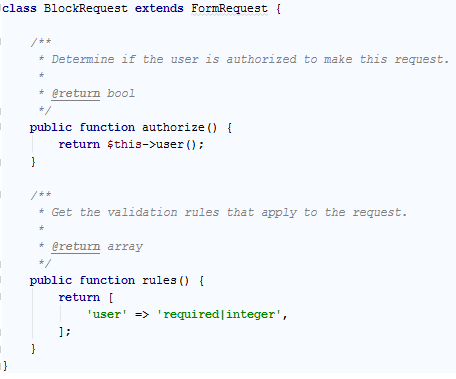
\includegraphics[width=\linewidth]{Images/Testing/BlockRequest}
\caption{Custom request for blocking users}
\label{fig:BlockRequest}
\end{figure}

Figure \ref{fig:BlockRequest} shows an example of one of the custom requests used for blocking a user. In this, we can see two functions: one for checking the authorisation of the user making the request and another which includes a set of validation rules. 

\subsection{Permission Testing}
Fidelis is split into accessible pages for authorised and unauthorised users. As such, permissions for page access and actions permissible for a user needed to be tested. This form of testing is important as it deals with the protection of users and their data. The first portion of this testing involved looking at pages that should only be accessible to authorised users. Functionality for checking user authorisation was done by the authentication middleware, but this was tested to make sure it was applied correctly. The remainder of permission testing dealt with verifying requests on a per user basis. This involved checking that a user was permitted to perform the operation they were attempting. For example, user $B$ should not be able to edit or delete posts made by user $A$. Additionally, only user $A$ should be able to modify their settings.

\section{User Acceptance Testing}
User Acceptance Testing (UAT) is one of the last stages of the software development lifecycle, and is performed on the end-user of a given product to gain feedback and approval on the final product \cite{EconomicTimes:UAT}. UAT is an important part of overall testing and from it, it is possible to identify bugs and gain useful insights into the system and how users view it. This section will look at how UAT was conducted for this project, and in particular, will focus on the feedback received from users.

\subsection{User Feedback}
The entire system relies on a stable and growing user base; without the users, the system would be rendered useless. With this in mind, guaranteeing a more than satisfactory user experience was integral to system success, and it was, therefore, important to gain feedback on the user experience offered by Fidelis. By correctly analysing feedback received from users, system strengths and weaknesses could be identified for each progressive system prototype. A number of users were consulted after being given access to the system at various stages of development in order to identify any issues that users may have with the system so that these could be dealt with in later development stages.

Throughout the development of the system, users were given questionnaires along with a list of tasks to complete. Once the users completed each task, they would answer the questions corresponding to the tasks. No guidance was given to the user and they were expected to use their intuition to navigate the system and perform the tasks. The survey not only included questions on system navigation but also had questions related to UI design, recommendations and settings provided for privacy and security. Figure \ref{fig:UATQuestionnaire} shows part of the survey given to users after development was completed. The survey accepted a combination of multiple choice and written answers. Multiple choice questions were used to gauge overall user consensus, whereas as written answers provided more detailed feedback on specific system components.

\begin{figure}[H]
\centering
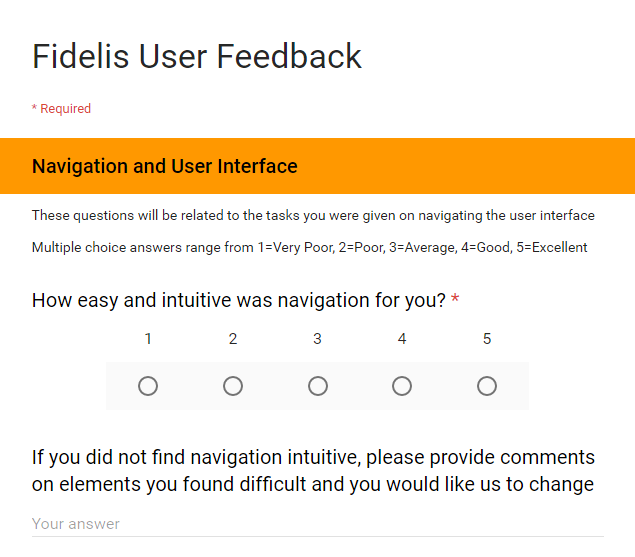
\includegraphics[height=3in]{Images/Testing/UATQuestionnaire}
\caption{Section from final questionnaire given to users as part of UAT}
\label{fig:UATQuestionnaire}
\end{figure}

As mentioned previously, Fidelis design adopted a lot of design elements from Twitter. As a result of this, users felt very comfortable navigating through and using Fidelis. Feedback received, mostly orally, highlighted that the system did need to re-design elements of the UI as it felt and looked too similar to Twitter. A discussion of UI re-design is included in Chapter \ref{Chapter:Conclusion}. Users were very receptive towards the idea of controlling how recommendations were generated for them. By being able to specify a method for recommendations, users were enabled to buy into the idea of Fidelis being a platform that enables them to engage with content they are interested in and have control over. Similar sentiments were voiced on the ability to fine-tune how abuse detection and reputation scoring was conducted.

Acceptance testing played a key role in the development process of the system. Prototypes were built and presented to the user which they evaluated and the feedback from the users was then incorporated into the next iteration of the system. Often a different selection was used to provide an unbiased feedback as existing users would be familiar with the system after previous tests. However, on the final acceptance testing of the complete system, a mix of new and existing users was required to test the system to see what new users thought about the final product as well as how existing users thought the system had improved.

\subsection{Testimonials}
In this section, we look at some of the testimonials received from users. Testimonials were important to collect as they not only give attestation to the success of the system but also offer up constructive criticisms that will be useful for further system development.

\begin{displayquote}
    \enquote{It's really interesting how Fidelis is aiming to tackle the issues which exist in social networking. It is definitely a site I would be interested in using, although it will be difficult for it to replace the big names such as Facebook and Instagram in terms of marketing.}
    
    - Elenya McCue, \textit{Engineering BEng, University of Warwick}
\end{displayquote}

\begin{displayquote}
    \enquote{Fidelis is the whole package. A clever idea backed up with a clean and intuitive design. Aside from the stark similarity to Twitter this idea can definitely go places.}
    
    - Joshua Greenwood, \textit{Advanced Computer Science MPhil, University of Cambridge}
\end{displayquote}

\begin{displayquote}
    \enquote{The design is sleek, clean and familiar. The more I use it, the more posts interest me. It's like it knows me} 
    
    - Luke Vincent, \textit{Graduate Technology Analyst, Barclays PLC}
\end{displayquote}

\begin{displayquote}
    \enquote{Fidelis seems like a different kind of social network. The features it has would allow people to have better interactions compared to other networks like Facebook or Twitter and stop anyone from seeing anything they wouldn't want to. I guess the next step is how you guys plan on making money from this?}
    
    - Hannah McAloone, \textit{Chemistry MSC, University of Warwick}
\end{displayquote}

\noindent The testimonials above, collected from a diverse group of individuals highlight the potential Fidelis has as a product that can disrupt and innovate in the current social network market. 
\chapter{Project Management}
\label{Chapter:ProjectManagement}
Due to the extensive length and size of this project, consideration into how the project can be effectively
managed was very important to project success. The following sections will discuss the chosen design and development methodologies, providing justification for each choice and will also look at the risks affecting project progress and success.

\section{Design Approach}
The design approach adopted for system UI was component-driven design. Component-driven design allowed more focus and thought to be given for each component. Going with this approach was greatly beneficial to the project as it meant components were designed independently of each other. Another advantage of using this methodology is that it provides the opportunity to re-use designed components across multiple applications. Using component-driven design ties in well with \textbf{NF5} from Chapter \ref{Chapter:SystemRequirements}. Using this design approach, system components are designed independently of one another allowing for extensibility and easy modification.

For algorithm design, an Agile approach was used. Agile methodologies provided flexibility when researching and designing chosen algorithms. Over the course of the project, numerous algorithms were considered and with the flexibility provided by this approach meant any required changes to algorithm design were prompt.

\section{Software Development Methodology}
Agile methodologies were employed for project development. This, coupled with component-driven design meant enabled components to be designed, built and tested seamlessly. Agile techniques were used due to their flexibility in handling evolving requirements. Due to the project length, it was important to adopt an adaptive development methodology. Building the system using Agile techniques eases the integration of new system components, and increases the efficacy of unit testing. Another reason that an agile approach was chosen was that as development progresses, issues will arise which may not have been accounted for previously. Adapting to these issues, and evolving requirements would not be possible with a plan-driven approach such as Waterfall. Given their linear nature, requirements refinement is much more difficult hence an agile approach provides a way of handling changing requirements. 

One fact that must be brought to light is that agile methodologies do not focus on documentation as much as a plan-driven approaches. As documentation is a key part of the non-functional requirements of this project, a modified version of the agile approach, one where documentation is important, was used. In addition to this, rapid prototype development was also employed to cope with the overlapping of development and testing, allowing for quick component prototypes to be created and tested. To counteract the effects of reduced documentation, regular meetings were held with with project supervisor to ensure that project goals remained on track. Similarly, within the project group itself weekly meetings were held. Much like daily scrums, these meetings again reinforced project goals and provided a platform where next steps and progress blockers could be discussed.

\section{Project Timeline}
The proposed project timeline, composed during the project specification and visible in Figure \ref{fig:timeline} has remained largely unchanged. Given how the timeline was designed, providing generous float time to each activity, few minor changes were made to the original plan. To accommodate for the increased workload faced by team members in Term 2, work on the final report was delayed until March. Although this at first seems like a major delay, the 14 week period initially assigned for writing this report was purposefully made longer than required to accommodate for unforeseen circumstances that would affect the task. Subsequently, draft completion dates and feedback cycles were also pushed back. The implementation for each algorithm ran longer than originally planned. This again did not affect the overall plan as these tasks were already overlapping and as each algorithm was implemented by a different team member, full task parallelisation was possible, meaning the completion date for the final algorithm was successfully met.

\begin{figure}[H]
  \centering
  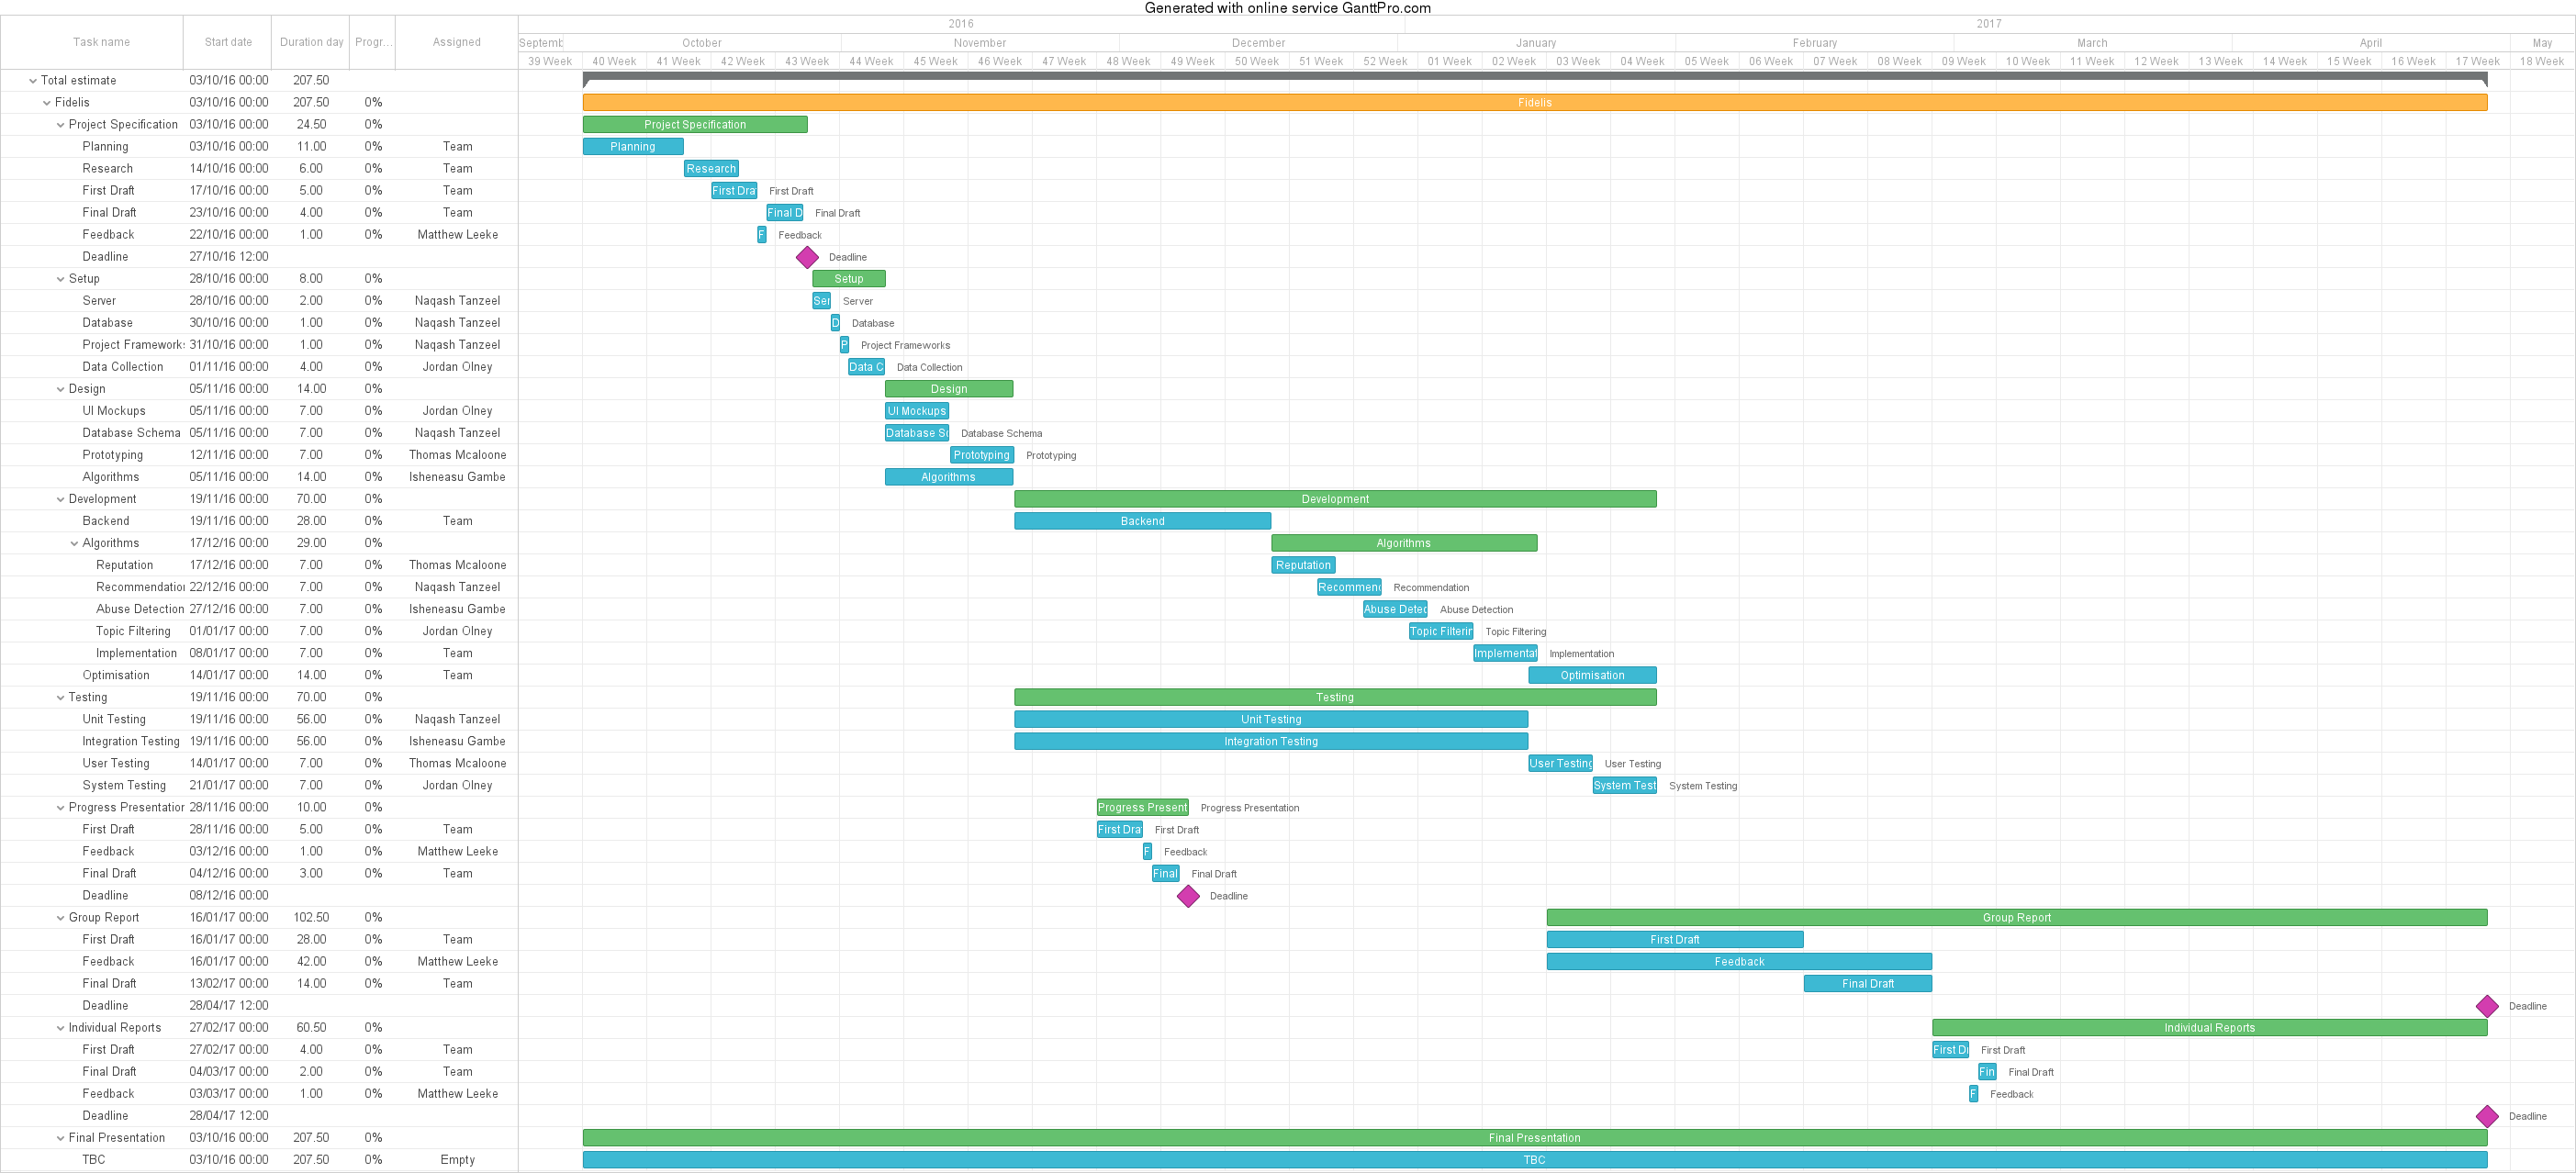
\includegraphics[width=1.0\textwidth]{Images/ProjectManagement/timeline}
  \caption{Project timeline} 
  \label{fig:timeline} 
\end{figure}

\section{Tools and Techniques}
A range of third-party tools and technologies were employed to successfully manage and develop the project. These tools have an immense amount of support and resources available online. As a result less time is spent `firefighting', solving issues, and `reinventing the wheel', hence allowing more time to be spent on developing the unique aspects of the projects. Using existing frameworks and tools also provides the added benefit that fundamental features and functionality is implemented by the third-party provider but can be taken advantage of by the developer. The tools employed were used for different tasks, either for developing the project or managing it to ensure a smooth operation, each of which are discussed in further detail below.

\subsection{Development}
\begin{figure}[H]
	\centering
	\begin{subfigure}[t]{0.2\linewidth}
		\centering
		
\includegraphics[width=\linewidth]{Images/Generic/Icons/Laravel}
		\caption{Laravel 5}\label{fig:Laravel}		
	\end{subfigure}
	\quad
	\begin{subfigure}[t]{0.2\linewidth}
		\centering
		
\includegraphics[width=\linewidth]{Images/Generic/Icons/HTML_5}
		\caption{HTML 5}\label{fig:HTML_5}
	\end{subfigure}
    \quad
	\begin{subfigure}[t]{0.2\linewidth}
		\centering
		
\includegraphics[width=\linewidth]{Images/Generic/Icons/CSS_3}
		\caption{CSS 3}\label{fig:CSS_3}
	\end{subfigure}
    \quad
	\begin{subfigure}[t]{0.2\linewidth}
		\centering
		
\includegraphics[width=\linewidth]{Images/Generic/Icons/JavaScript}
		\caption{JavaScript}\label{fig:JavaScript}
	\end{subfigure}
    \quad
	\begin{subfigure}[t]{0.2\linewidth}
		\centering
		
\includegraphics[width=\linewidth]{Images/Generic/Icons/PHP_7}
		\caption{PHP 7}\label{fig:PHP_7}
	\end{subfigure}
	\quad
	\begin{subfigure}[t]{0.2\linewidth}
		\centering
		
\includegraphics[width=\linewidth]{Images/Generic/Icons/MySQL}
		\caption{MySQL}\label{fig:MySQL}		
	\end{subfigure}
	\quad
	\begin{subfigure}[t]{0.2\linewidth}
		\centering
		
\includegraphics[width=\linewidth]{Images/Generic/Icons/jQuery}
		\caption{jQuery}\label{fig:jQuery}
	\end{subfigure}
    \quad
	\begin{subfigure}[t]{0.2\linewidth}
		\centering
		
\includegraphics[width=\linewidth]{Images/Generic/Icons/Apache}
		\caption{Apache}\label{fig:Apache}
	\end{subfigure}
	\caption{Development Tools Employed}\label{fig:DevelopmentTools}
\end{figure}

A wide range of technologies were used for the development of the project, some of which are shown in figure \ref{fig:DevelopmentTools}. Research into each of these technologies along with their advantages and disadvantages is provided in section \ref{Section:Technologies}. Section \ref{Chapter:Implementation} further discusses some of the core technologies such as Laravel, PHP, MySQL, jQuery and provides reasons for their use \cite{Laravel:Home, PHP:Home, MySQL:Home, jQuery:Home}. In addition to these core technologies, several smaller tools and technologies were also used. The majority of the user interface was developed using HTHML 5, although some of this was generated using the Laravel Blade engine, and styled using Bootstrap or custom Cascading Style Sheets \cite{W3:HTML5, Bootstrap:Home, W3:CSS}. Majority of the backend development was carried out using the popular scripting language PHP but some of this was also automatically generated using syntax provided by the Laravel Blade engine \cite{PHP:Home, Laravel:Blade}. 

\subsection{Management}
\begin{figure}[H]
	\centering
	\begin{subfigure}[t]{0.15\linewidth}
		\centering
		\includegraphics[width=\linewidth]{Images/Generic/Icons/PHPStorm}
		\caption{PhpStorm}\label{fig:PHPStorm}		
	\end{subfigure}
	\quad
	\begin{subfigure}[t]{0.15\linewidth}
		\centering
		
\includegraphics[width=\linewidth]{Images/Generic/Icons/Github}
		\caption{Github}\label{fig:Github}
	\end{subfigure}
    \quad
	\begin{subfigure}[t]{0.15\linewidth}
		\centering
		
\includegraphics[width=\linewidth]{Images/Generic/Icons/DigitalOcean}
		\caption{DigitalOcean}\label{fig:DigitalOcean}
	\end{subfigure}
    \quad
	\begin{subfigure}[t]{0.15\linewidth}
		\centering
		
\includegraphics[width=\linewidth]{Images/Generic/Icons/Wunderlist}
		\caption{Wunderlist}\label{fig:Wunderlist}
	\end{subfigure}
    \quad
	\begin{subfigure}[t]{0.15\linewidth}
		\centering
		
\includegraphics[width=\linewidth]{Images/Generic/Icons/Trello}
		\caption{Trello}\label{fig:Trello}
	\end{subfigure}
	\caption{Management Tools Employed}\label{fig:ManagementTools}
\end{figure}

All the code written throughout the development process was done using an IDE provided by JetBrains called PhpStorm \cite{JetBrains:PHPStorm}. PhpStorm provides syntax highlighting, code completion, and numerous other features for all major web development technologies. Optional plugins can be installed which provide support for even more technologies, as done for Laravel \cite{JetBrains:PHPStorm}. PhpStorm also provides integrated support for Git which was used to provide version control for all the code written. This allowed files to be added to Git as soon as they were created so they would not be omitted from commits, causing inconsistencies \cite{JetBrains:PHPStorm}. The use of Github allowed code to be backed up online, in case of a hardware failure, so it could be replicated onto another machine easily \cite{Github:Home}. This was particularly useful when deploying the code from the development server to the production server hosted by DigitalOcean\cite{DigitalOcean:Home}. As soon as a feature was fully implemented, it could be pushed up to the Github servers allowing for the changes to be fetched by the production server just by issuing a single command. 

\begin{figure}[H]
	\centering
	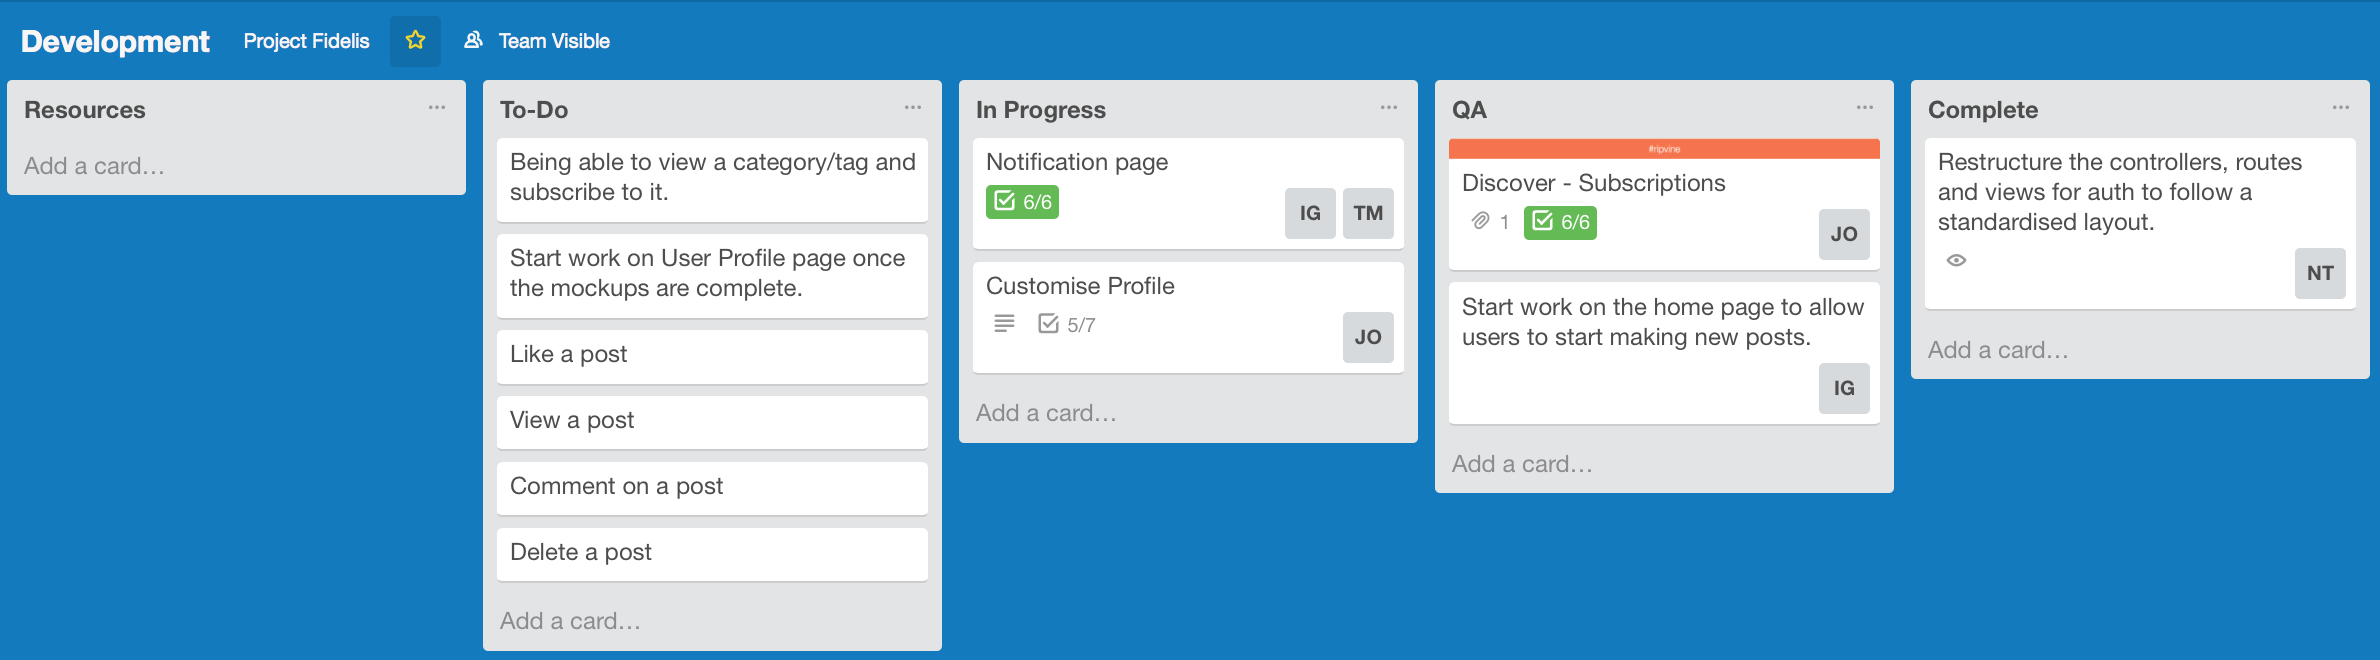
\includegraphics[width=1.0\textwidth]{Images/ProjectManagement/Trello}
	\caption{Trello: Project Work Breakdown Structure} \label{fig:Trello_WBS}
\end{figure}

A number of desktop and web applications were used to keep track of the daily development progress and any remaining work that needed to be completed. Wunderlist was used to keep track of daily tasks that needed to be completed whereas Trello, was used to keep an overall development log of all the features that were to be implemented \cite{Wunderlist:Home, Trello:Home}. Figure \ref{fig:Trello_WBS} shows just one of the boards, namely development tasks, used to keep track of progress. These were strictly for the developer and hence to communicate this progress, emails and face to face meetings were used to update the project supervisor and stakeholders. All the tools discussed are illustrated in figure \ref{fig:ManagementTools}.

\section{Risk Management}
Undertaking a project of this length, with the given time-scale and the nature of any software development project it was imperative that proper risk management be conducted to minimise major risks affecting project completion. Risks affecting developers, software, hardware, data and third party services were considered and mitigated against.

\subsection{Developer}
Project developers are crucial to project success. As with any software development project, the importance in understanding and managing risks that may affect developers cannot be undervalued. One of the main risks affecting any developer is their ability to perform the tasks they are assigned to. Illness, commitments to other work assignments or an inability to complete a given task can severely hinder project progress. To prevent any such occurrence, all developers were paired so that in the event that developer $A$ was unable to complete a task, developer $B$ would be able to understand and complete this task. Going beyond this, it was highly encouraged amongst the team to be aware of what other members were working on. This essentially meant that any developer was able to pick up tasks being handled by another developer. Additionally to this, effective communication channels were established within the team. This supported the idea of paired development as it made it easy for developers to work together, and also meant that potential issues were swiftly identified and dealt with. (VPS STUFF)

\subsection{Hardware}
All development has been done using personal computers, so the only hardware relied upon during the project were these devices. Along with other work and personal use, each device was used heavily, and was therefore prone to failure. To mitigate against this, version control software was used to maintain functioning back-ups of all development work. Namely, Github was used for this purpose. Github allows ``snapshots'' of the functioning system to be taken, making data retrieval in the event of hardware failure very convenient and easily. In addition to this, each developer kept a copy of their work on the Computer Science Department lab machines. These two approaches covered the occurrence of single and multiple device failure.

\subsection{Data}
Data security is important to any project where user data is collected. Exposing user data could leave the system and developers liable to penalties or criminal charges from relevant regulatory bodies. For this reason, it is important to ensure that in the case that user data is exposed, safeguards are in place to protect both the users and developers. To avoid storing plain-text user credentials, user passwords are hashed before being stored in the database, making it almost impossible for anyone to decrypt the data within a reasonable period of time. During the registration process, minimal information is requested from the user. When registering, the only information requested from the user is their name and email address. This minimal approach on user information lessens the amount of sensitive data held on users. Password-protecting the database added an extra layer of database security, minimising the chances of unauthorised access to any of the data.

Another piece of data that needs to be protected is any content that is uploaded by the user. Public user profiles are accessible to anyone on Fidelis, even to unregistered users. To provide users with the option of increased privacy, the user has the option to make their account private. This makes their content accessible only to their followers.

\subsection{Third Party Services}
The Twitter API is used to collect data for training a model for automatic post categorisation. This falls under content filtering, one of the core Fidelis functionalities. Were this service to fail, it would make the process of collecting training data very difficult and cumbersome. In the event that such a failure would occur, alternative datasets were collected. A number of public datasets for natural language processing are available online. The Blog Authorship Corpus is a public dataset containing 681288 blog posts from 2004 \cite{dataset:blogs}. This, along with several other datasets \cite{dataset:all} were available as fall-back training datasets.

The API has a rate limit on the number of tweets that can be fetched, permitting 180 tweets per 15 minute window \cite{twitter-api:rates}. This rate puts a restriction on how many tweets can be collected daily, and inefficient tweet collection can therefore lead to not enough data being collected. This would in turn hamper the training of the model. To maximise the number of tweets collected, data collection began early on in the project and a DigitalOcean droplet was setup, allowing automated data collection on the server.

\chapter{Evaluation}
\label{Chapter:Evaluation}
After a comprehensive look at system design, implementation and testing, focus now turns to performing an evaluation of how well the completed system aligns with the original, envisioned idea. To this end, system requirements will be evaluated to assess how closely they met the requirements set out in Chapter \ref{Chapter:SystemRequirements}. Assessment will occur as a pass-fail test, coupled with a brief comment on each requirement. Additionally an evaluation of the legal, social, ethical and professional issues affecting the project, discussed in Chapter \ref{Chapter:Issues}, will also be provided.

\section{Requirements}
This section of the report will look at both functional and non-functional requirements. Evaluation of each requirement, as set out in Chapter  \ref{Chapter:SystemRequirements}, is done using a pass-fail test. Along with tables detailing evaluation results for functional and non-functional requirements, the following sections will also provide justification for any requirements that have not been met.

\subsection{Functional Requirements}
Table \ref{tab:functional-eval} shows the results from functional requirements evaluation. This is essential in identifying whether the product has met its goals and provides the functionality set out by the project stakeholders. All functional requirements set in the project specification, and later refined, were met; the system adheres to and is capable of performing all of the desired functionalities. 

\begin{longtabu} to \textwidth {XXXX}
\hline
Requirement & Description & Comment & Result \\ 
\hline
\textbf{F1} & The system must be able to communicate with a number of third party APIs in order to retrieve data & The Twitter API is used to retrieve tweets that are used to train the classifier for automatic post categorisation \vspace{2mm} & \textcolor{passgreen}{PASS} \\
\textbf{F2} & Users must be able to register and log into the system & The system allows for users to register as a new user or log in as an existing user \vspace{2mm} & \textcolor{passgreen}{PASS} \\
\textbf{F3} & A user may make their account private, preventing other users from being able to see the content they share & Users have the option to toggle privacy on their accounts. All accounts are public by default \vspace{2mm} & \textcolor{passgreen}{PASS} \\
\textbf{F4} & A user may block another user & Users have the option to block other users using a `block' button \vspace{2mm} & \textcolor{passgreen}{PASS} \\
\textbf{F5} & In order to see content, users should be able to add other users to their ``trust circle'' \vspace{2mm} & Users can add to their ``trust circle'' by following other users & \textcolor{passgreen}{PASS} \\
\textbf{F6} & The system will overcome the cold-start problem, under which a user will not see anything on their timeline upon registration, by providing a set of predefined categories which can be used to explore &                                                                                            Fidelis has the following default categories, available to the user as soon as they register: Education, Fashion, Finance, Fine Arts, Food, Health, Home, Miscellaneous, Politics, Politics, Sport and Travel technology \vspace{2mm} & \textcolor{passgreen}{PASS}  \\
\textbf{F7} & The system will provide a personal feed where the user is able to view content from the people they trust, prioritised by the reputation of the people they follow as well as the reputation of the content itself  \vspace{2mm} & Each user has a feed for the users they follow. This feed contains content from these users which is ranked by reputation of the author and their content & \textcolor{passgreen}{PASS} \\
\textbf{F8} & A user must be able to post new content to the system                                                                                                                                                              &   Users are able to post new content on the homepage. When submitted, this post is appended to the users' personal feed. Within the post, the user can mention specific individuals by using their username preceded by an @ symbol \vspace{2mm} & \textcolor{passgreen}{PASS} \\
\textbf{F9} & Users can view any posts made by public accounts or by private accounts which they follow & Users can only view posts made by a public account. To be able to view content from private accounts, users must first make a request to follow the private account \vspace{2mm} & \textcolor{passgreen}{PASS} \\
\textbf{F10} & Users must be able to reply to a post made by another user &  Users can reply to a post in a similar manner to when posting new content. When a comment is made, the author of the post is notified of this. Replying to a post starts a thread of comments akin to Facebook commenting. Within comments, users can mention specific users. This also notifies the relevant user \vspace{2mm} & \textcolor{passgreen}{PASS} \\
\textbf{F11} & Users may interact with content they come across by liking or disliking it. Each of these actions will impact the reputation of the content \vspace{2mm} & The user can like and dislike posts by using the thumbs up and down icons which accompany every post & \textcolor{passgreen}{PASS} \\
\textbf{F12} & Users are notified of any collaboration events involving their account & The user receives a notification whenever another user requests to follow them, or whenever their content is liked, disliked or commented on \vspace{2mm} & \textcolor{passgreen}{PASS} \\
\textbf{F13} & Users may change the appearance of their post & The user is able to upload their own personalised profile picture and cover picture to appear on their profile and throughout Fidelis \vspace{2mm} & \textcolor{passgreen}{PASS} \\
\textbf{F14} & The system will automatically calculate a reputation score for users which symbolises the trustworthiness of the user and the content they post & Using an abuse detection classifier, along with a script that calculates post reputation, user reputation will be determined by the content they post on Fidelis \vspace{2mm} & \textcolor{passgreen}{PASS} \\
\textbf{F15} & The system will also calculate a reputation for each user posted content to represent the quality of content & A Python script, which is run periodically, will retrieve user posts and calculate the reputation for each post based on the votes on it. Additionally, if a post is deemed abusive its reputation will reflect this \vspace{2mm} & \textcolor{passgreen}{PASS} \\
\textbf{F16} & Each user will be able to choose how the notion of trust is implemented & Users are able to toggle between multiple representations of trust \vspace{2mm} & \textcolor{passgreen}{PASS} \\
\textbf{F17} & The system will provide recommendations to the user & User and content recommendations are generated for users. User recommendations are available through a widget across the home and profile pages, and content recommendations are available on the discover page \vspace{2mm} & \textcolor{passgreen}{PASS} \\
\textbf{F18} & The system will allow the user to choose how recommendations are generated for them & Users are able to toggle settings related to how recommendations are generated for them. Namely these are the reputation of users and content, the number of recommendations to generate and a similarity threshold \vspace{2mm} & \textcolor{passgreen}{PASS} \\
\textbf{F19} & The system will incorporate abuse detection to prevent things such as profanity, swearing and nudity amongst other things & Fidelis has in place an abuse detection classifier that is able to detect abusive content. Similarly to the script calculating reputations, the classifier will be run periodically on user posts. Users are also able to manually report content they find offensive \vspace{2mm} & \textcolor{passgreen}{PASS} \\
\textbf{F20} & Users can report content which they find is inappropriate or offensive, such as profanity or nudity                                                                                                                &  Users can flag posts they find inappropriate using the flag icon that accompanies each post. Flagged items are used to re-train the abuse detection classifier to increase its accuracy in detecting abusive content                                                                                             \vspace{2mm} & \textcolor{passgreen}{PASS} \\ 
\hline
%\end{tabular}
\caption{Evaluation of Functional Requirements}
\label{tab:functional-eval}
\end{longtabu}

\subsection{Non-Functional Requirements}
Non-functional requirements ensure that the developed solution is applicable to usage in the real word. Functional requirements may ensure that the system provides all the features required, but these could be entirely useless if the system is not user friendly. Table \ref{tab:nonfunctional-eval} discusses all the non-functional requirements and how closely these requirements were met. The comments column discusses how the requirement was met and whether any aspects of the requirement were missed. As visible in the table, all requirements were passed; the system goes beyond just being functional and additionally meets, amongst other things, criteria set for usability, scalability and extensibility.

\begin{longtabu} to \textwidth {XXXX}
\hline
Requirement & Description & Comment & Result \\ 
\hline
\textbf{NF1} & Compatibility & Fidelis is compatible across all devices. Using Bootstrap for front-end development, cross-platform compatibility was guaranteed. System functionality is compatible for mobile devices, but some features may be hidden \vspace{2mm} & \textcolor{passgreen}{PASS} \\
\textbf{NF2} & Usability & The decision to imitate Twitter UI design meant that the system inherited designs that have been refined over time to provide a good user experience \vspace{2mm} & \textcolor{passgreen}{PASS} \\
\textbf{NF3} & Security & All data held by Fidelis is stored in a password-protected database. Additionally, user credentials are encrypted when stored. The option to make user accounts private add an additional security layer to protecting user data \vspace{2mm} & \textcolor{passgreen}{PASS} \\
\textbf{NF4} & Scalability & Whilst all decisions taken have been taken with storage and processing power in mind, larger datasets may result in slow response from the system on the current hardware. Due to the fact that users are allowed to upload resources, it is difficult to contain storage within a limit and hardware upgrades will be necessary as the system grows. It is also impossible to test this requirement without a large user base \vspace{2mm} & \textcolor{passgreen}{PASS} \\
\textbf{NF5} & Extensibility                                                                                                                         & The system was developed using a modular approach made possible through the use of an MVC approach. This means that the system can be expanded at any time as each module is completely independent of another and can be upgraded or replaced with ease. This also allows new functionality to be integrated into the system with ease \vspace{2mm} & \textcolor{passgreen}{PASS} \\
\textbf{NF6} & Maintainability & The system is made maintainable by the documentation on all of the PHP code written throughout the project. Good coding practices as laid out by the frameworks and PHP manual were used. In addition, version control was used with through details provided for each commit. A regular update was performed for the Laravel framework to ensure that the latest version was being used. All third party apis use a CDN which means they're updated as soon as new version become available \vspace{2mm} & \textcolor{passgreen}{PASS} \\
\textbf{NF7} & Readability & As mentioned in maintainability, the code has been well documented. This is done only for the PHP code as the remaining code is relatively self explanatory. All changes were logged through version control as well as other progress tracking tools and a clear outline is provided in this report \vspace{2mm} & \textcolor{passgreen}{PASS} \\
\hline
\caption{Evaluation of Non-Functional Requirements}
\label{tab:nonfunctional-eval}
\end{longtabu}

\section{Legal, Social, Ethical and Professional Issues}
At the outset of this project, a number of legal, ethical, social and professional issues that could affect the Fidelis platform were identified. These issues were discussed fully in Chapter \ref{Chapter:Issues}. It is critical to review the issues discussed and identify how they have been addressed, and as such this section will look at these issues were confronted. In terms of legal issues, there could be concern that the content/activity of a user may have implications for Fidelis, for example a user posting copyright infringing content. It has therefore been outlined in the Fidelis Terms of Service that a user is responsible for their own content and activity on the Fidelis platform and also that any content deemed illegal may be removed. In order to comply with copyright law during development of the platform, it was ensured that each team member was made aware of the laws outlining which content could be used. The platform was developed largely using Laravel, an open-source php framework \cite{Laravel:Home}. The Fidelis logo is an original and so can be used with no permissions needed and other images and icons around the website were collected from open-source font libraries such as font-awesome \cite{FontAwesome}.

Social issues included the consideration of social networks and their relationship with mental health. It has been made clear that users should only post content they are comfortable with sharing to avoid users regretting doing so and the support section of the website suggests some ways a user can find help. This includes contact details and website of Samaritan's \cite{Samaritans:Home}, a charity providing assistance in talking over any issues a person may be having in their life and offering support to help that person overcome these issues. Additionally, the user may wish to change their settings for abuse detection. Our abuse detection system is designed to identify any content that the user may find abusive or offensive in any way and remove it. This ensures they only see content they wish to see. Unfortunately, this system cannot be relied upon fully, as occasionally there may be some content that an individual may take issue with which is not identified by the system as being abusive. In these cases, users can make use of the ability to report content. This will prevent them from seeing this content again and will affect the reputation of the content and the user that posted it, making it less likely that others will see the same content.

There are also ethical considerations for the Fidelis platform. It may be the case that users may not wish for everybody to see their posts. It has therefore been ensured that users can set their accounts to `private' on their settings page. This will prevent non-approved users from seeing the content they share. In addition there is the potential for the bias of any person(s) involved in the development of the Fidelis platform to affect the content recommended. Fidelis has been designed and implemented in such a way that content recommendation and filtering is based on user preferences as well as the content the user interacts with and they should primarily be shown content from other users that post `good' content, i.e., content/users with a high reputation. There is no reason that the views of anyone involved in developing the platform should affect the end-user content.

On a professional level it was noted that the Fidelis platform is required to adhere to the Data Protection of 1998 \cite{DPA}. In order to comply, it has been ensured that the database is as secure as possible. Sensitive data such as user passwords are encrypted to protect their information and any request to interact with data from the database (both retrieving and inserting data) requires checks such as ensuring the user is logged into an account and cannot interact with data related to another user. This way no individual can have access to data that they are not authorised to access, maintaining data confidentiality.

\section{Project Management}
The decision to use agile techniques for development, as discussed in Chapter \ref{Chapter:ProjectManagement}, enabled the project to evolve in parallel with changing project requirements. Using these techniques also provided developers with a creative freedom, which in itself played a hand in refining requirements. Adopting a ``custom'' agile approach that facilitated extensive documentation was a good idea. This addition to agile techniques introduced structure to the project. Changes made to the project timeline occurred, and are discussed again in Chapter \ref{Chapter:ProjectManagement}, but as mentioned these did not affect development work and were dealt with effectively due to chosen methodologies. The tools employed for both development and management were a success. Development tools were current and up to date, meaning all development work done will age well. The management tools used meant that all work was done transparently, and created multiple channels through which work could be discussed and evaluated. The risk analysis performed at the start of the project set it up to be able to cope with any minor or major risk. Fortunately, no major risks were realised. Few developer illnesses and unavailability plagued the project, but these events were planned for and handled effectively.
\chapter{Conclusion}
\label{Chapter:Conclusion}

\section{Summary}
The aim of this project was to provide a trust-based social network for user engagement and protection. The product realised at the end of this project provides a fully-functional social network. Not only this, but the delivered product also achieves its goal of being a trust-based social network. Through the use of abuse detection, user reputations and content filtering, user protection from abusive content or content they do not find interesting is ensured. With content recommendation, users can be sure that they will be provided with content and other users they will enjoy engaging with. This, along with meeting all the specified functional and non-functional requirements ensured that stakeholder satisfaction was guaranteed. 

The final deliverable goes beyond being just a minimum viable product, and instead exceeds the expectations set out at the beginning of the project.

\section{Future Work}
Balancing development work with academic commitments meant that amount of time dedicated to developing Fidelis was limited. As a result of this, although all functional requirements were met, more can still be done to improve Fidelis and take it beyond where it already is. To this end, a discussion will follow, looking at some of the ways the system can be improved upon.

\subsection{Improved User Interface}
Currently, the Fidelis UI is near identical to that of Twitter. This was a sentiment both applauded and criticised by users throughout UAT, as exemplified in the testimonials given by Vincent and Greenwood. A large part of future work should therefore focus on improving the current UI design. Although the design should be re-worked, users did enjoy the familiarity of design with Twitter so some aspects of the UI should be retained. What is retained and changed is left at the discretion of future developers.

\subsection{More Complex Reputation Scoring}
The reputation scoring system currently implemented is very simple. To provide users with up-to-date reputations, it was decided to implement a computationally fast algorithm. The trade-off as a result of this decision means that some might deem the complexity of scoring insufficient. However, the voting system chosen, although simple, has been proven to be effective given its use by Reddit and Youtube \cite{Reddit:About, Youtube:Home}. Nonetheless, this system can be prone to bias, which we see with likes on YouTube. A video can be of good quality, but if users do not like the author of the video e.g. most videos related to Justin Bieber, votes won't reflect the quality of the content. The weighting system used avoids this to an extent, but more complex techniques can be used. Future work should therefore involve researching algorithms that can perform quick reputation scoring, whilst using more complex techniques that will only improve upon current scoring mechanisms.

\subsection{Classifier Refinement}
The data used for model training and evaluation was collected from Twitter and other resources. As a result of this, the size of the dataset was limited and dated. To provide better performing models, classifiers should be re-trained with new user data once the network becomes more active. By re-evaluating models with current data, the dataset used for training will be larger, leading to potential performance improvements. Given more time, model fine-tuning should take place with more in-depth parameter searching. This could again improve model performance. Another refinement which could be made to tag categorisation model is to train this model on individual tags rather than entire posts, in order to improve the performance of the system in this area. This would require a large enough training set of tag-category pairs with which a model would be able to learn.

\subsection{News Recommendations}
One of core functionalities discussed throughout the report has been providing users with recommendations. This functionality was successfully implemented, but the system should not limit itself to just the current forms of recommendations. An idea that was discussed during development was to provide users with news articles relevant to what they post.
This piece of work would involve attaching news stories to a users' post that are related to the topic of the post. Facebook currently provides trending news stories, but these articles may not always be of interest to the user. The driving factor behind this concept is to again provide engaging content to the user. This work would also help in reducing the echo chamber effects as articles provided would only be related to the topic of the users posts, and not necessarily reflect their own sentiment.

\subsection{Additional Social Network Functionality}
Existing social networks provide a standard set of ``expected'' functionality. Common things included in this are sharing posts, posting videos and user messaging services. The aim of Fidelis was to tackle the downfalls of existing platforms by providing a novel solution addressing these issues, but as the focus was on this the final product failed to implement the aforementioned functionalities. Therefore, any future work on the system should include integration of the these functionalities. Providing these functionalities would broaden channels through which users can engage with content and each other.

\bibliography{referencing/bibliography}
\bibliographystyle{plain}

\renewcommand{\appendixpagename}{\centering Appendices \clearpage}
\long\def\appendixsection#1{\centering\section{#1} \clearpage}

\begin{appendices}
\appendixsection{Project Specification}

\includepdf[pages={-}]{appendix/Specification}

\appendixsection{Progress Report}

\includepdf[pages={-}]{appendix/ProgressReview.pdf}

\appendixsection{Presentation}
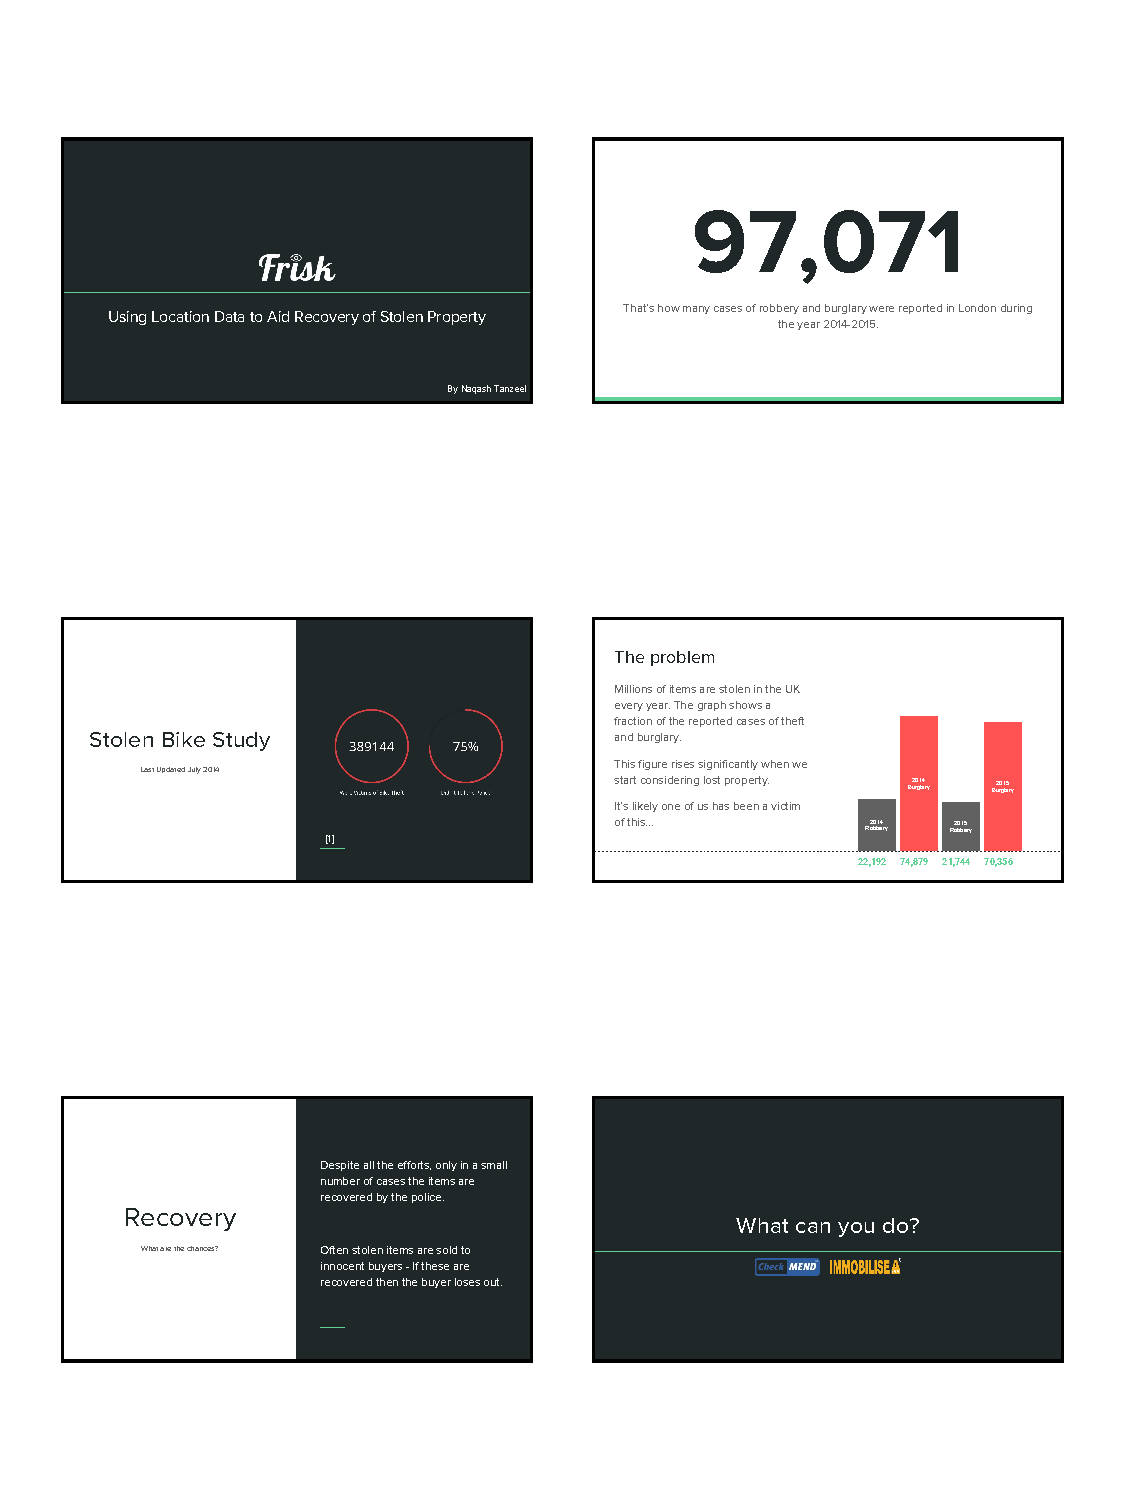
\includepdf[pages={-}]{appendix/Presentation.pdf}

\appendixsection{Quick Start Guide}
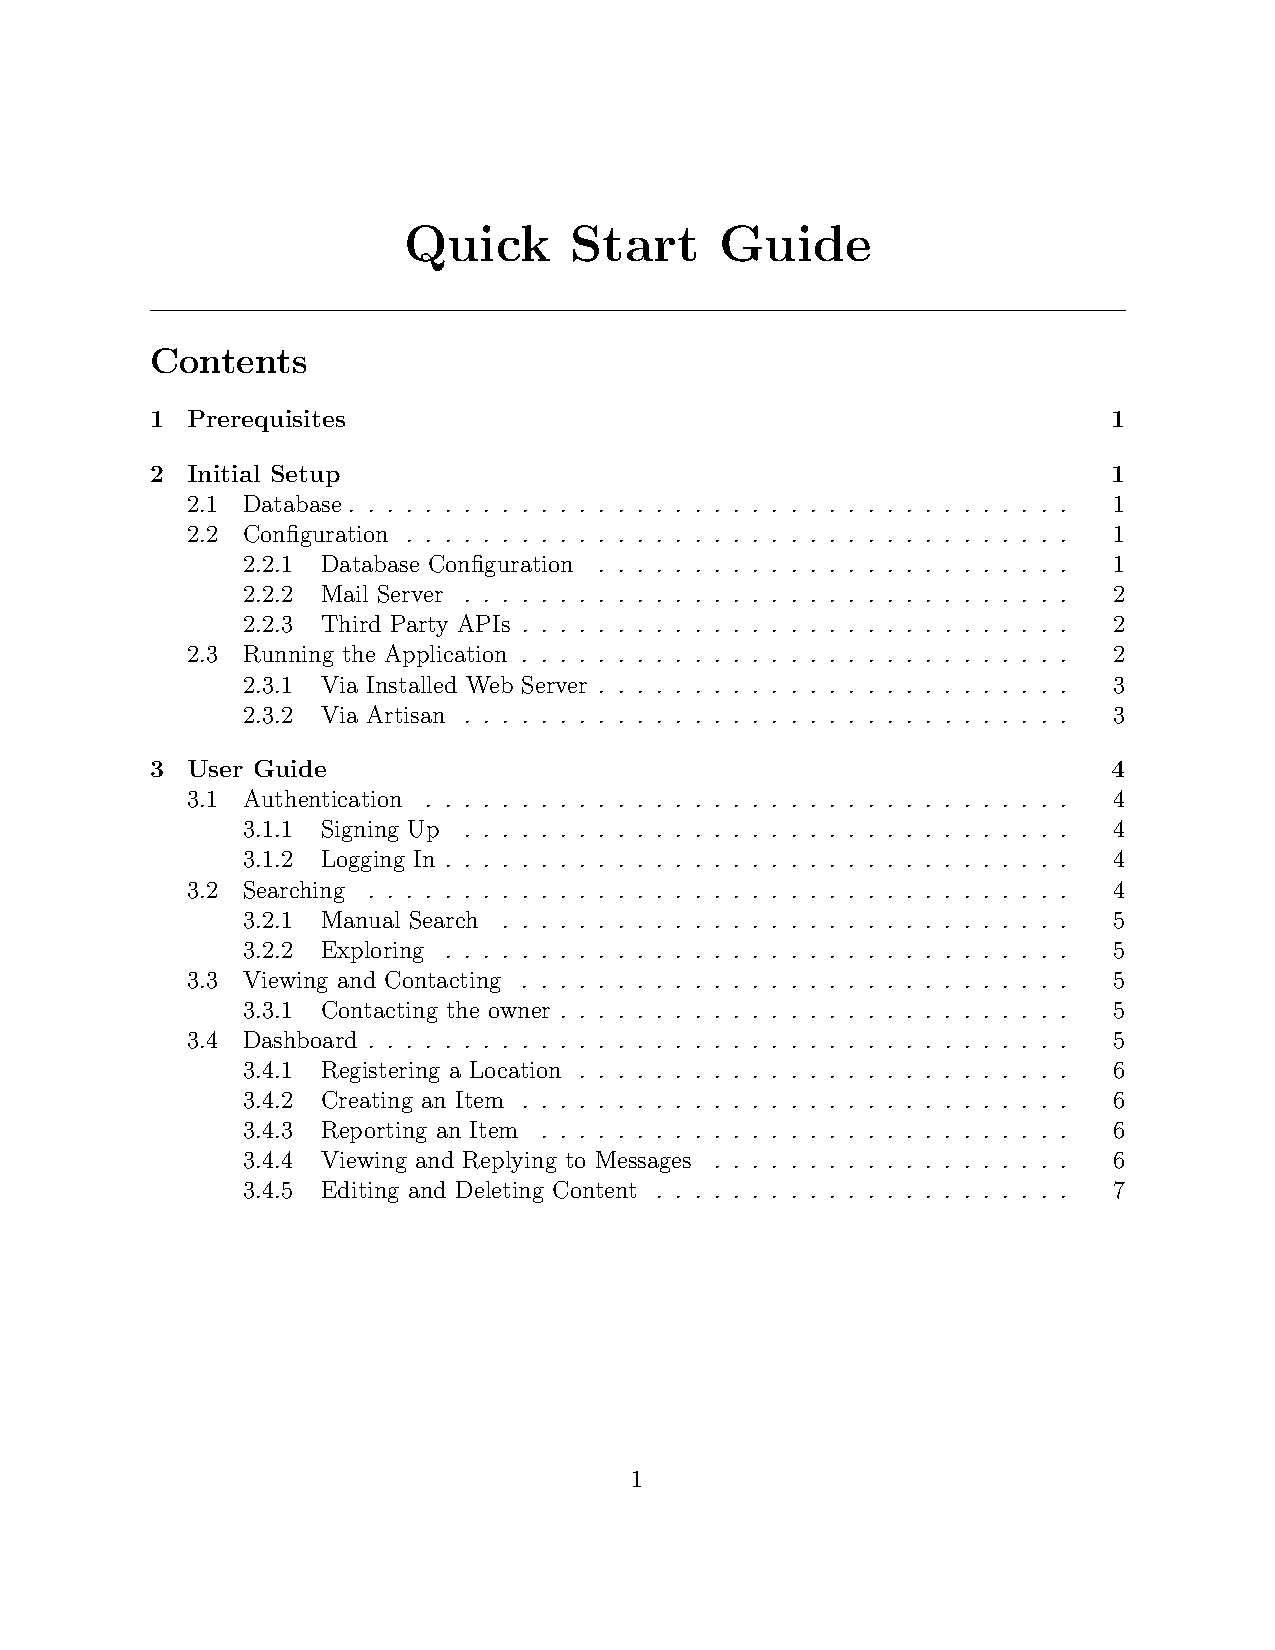
\includepdf[pages={-}]{appendix/Guide.pdf}

\end{appendices}

\end{document}